\chapter{Parallelization}
\label{chap:parallel}

%\epigraph{%
%Demonstration is made of the continued validity of the single processor approach
%and of the weaknesses of the multiple processor approach in terms of application
%to real problems and their attendant irregularities.}{Amdhal (1967)}

\section{Introduction}
\subsection{Architectures}
\label{subsec:architectures}
\glspl{CTM}, and in a larger measure climate and weather models, are
CPU-consuming applications, where the performances are usually quantified using
the number of \gls{flops}. As such, they benefited greatly from the improvements
in microprocessor architectures, usually described by Moore's law. Two
consequences of this law for single-core microprocessor are the decrease of
transistor area and transistor delay. Up to 2004, the increase in clock
frequency was kept in check by the decrease in the operating voltage so cooling
the chip was still rather inexpensive. It is no longer the case after 2004. 
Power is now a scarce resource so new processors aim for a better performance
per unit power. For performance, the current limiting factor for microprocessor
is memory bandwidth and latency and new designs are being studied to attempt to
deal with that.  Therefore, designing scalable applications must take into
account the cost of memory accesses.

The current micro-architectures can be divided into three categories. The first
contains `conventional' microprocessors which focus on improving the
performances of single \glspl{thread}, such as AMD's K8 core. Another
approach is taken by Sun for its Niagara 2 chip where multiple threads are
chosen over single-thread performance. \\
In the second category, we have \glspl{GPU}, which were initially designed for
graphics rendering but are now used for general computations. Their design is
fundamentally different from \glspl{CPU}. CPUs aim at decreasing latency, for
example with larger caches (memory latency), branch prediction (branch latency)
and better arithmetic and logic operation (operation latency). GPUs aim at
improving the throughput using smaller caches for example. More energy-efficient
than CPUs, they however are better suited for large number of truly independent
tasks. NVIDIA is the most popular GPU constructor at the moment and their latest
(2013) Kepler GPU have 15 multiprocessors with 192 cores each
(\cite{nvidia2012}).\\
Multi-core microprocessors make the third category. They emerged from the
limitations of single-core microprocessor and stack on the same chip several
cores. As an example of application, in pure MPI programming, a parallel task is
associated to a single core. These microprocessors can be further divided into
categories according to the communication between cores.  The most common design
is a `tree' of different level of caches, with access to the main memory as the
top as illustrated on Fig.~\ref{fig:bull_processor}.  More details and other
designs can be found for example in~\cite{Kogge2008}.

\defcitealias{Top500}{Top 500 website}%
However, a single instance of one of these architectures is not sufficient for
massively parallel applications, which require tens or hundred of thousands
tasks. To achieve that, supercomputers are used in practice, where
several `computing nodes' are connected together via a fast network to create a cluster.
Nodes can be designed specifically for parallel computation, such as the vector
processors in the Earth simulator but the majority of clusters uses
`commercial' nodes, \textit{i.e}, with mass-produced hardware. In practice, a
node contains one or more microprocessors (multi-core or not) or GPUs in some
cases. More details about the current architectures can be found in the
\enquote{Top 500}, which lists the most powerful supercomputers of the world twice a year
(see the~\citetalias{Top500}).\\
As an example of a cluster, the configuration of the Bull cluster at CERFACS
(used later in the chapter) is shown on Fig.~\ref{fig:bull_cluster}. It can be
seen that each node shares a large amount of RAM for its processors but there is
no global address shared across the nodes. From the point of view of the nodes,
we have a \textit{distributed-memory} model. However, at the level of the processor, we
can have a \textit{shared-memory} model.  While these are the two main architectures,
it should be noted there is an effort to use a global address space, the
\gls{PGAS} model. One implementation of this model is the \gls{UPC} language
(see~\cite{Carlson1999}).  The choice of the programming model then depends on
the memory architecture as explained below.

\begin{figure}
  \subbottom[Memory hierarchy in the 8 cores of a Sandybridge processor. L1
  and L2 are local to the cores (32KB and 256 KB resp.), while L3 (20MB) is common to
  the 8 cores. L1 is the small and fastest cache, while L3 is the largest but
  slowest.]{%
    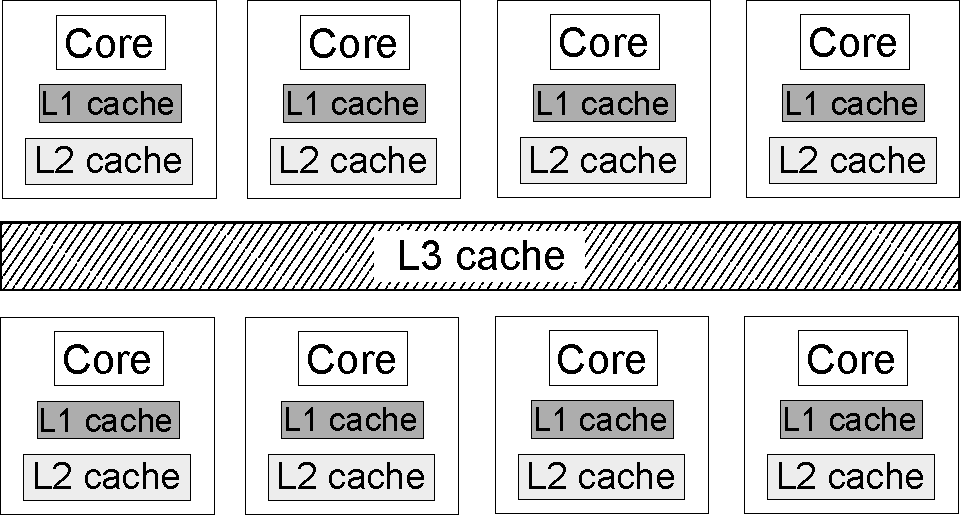
\includegraphics[width=0.48\linewidth]{sandybridge.pdf}
\label{fig:bull_processor}}
  \hfill
  \subbottom[4 nodes of the clusters are shown here. Each node has 2 Sandy
  Bridge processors sharing 32GB of RAM\@. Nodes are interconnected with an
  Infiniband network with a speed of 5GB/s.]{%
    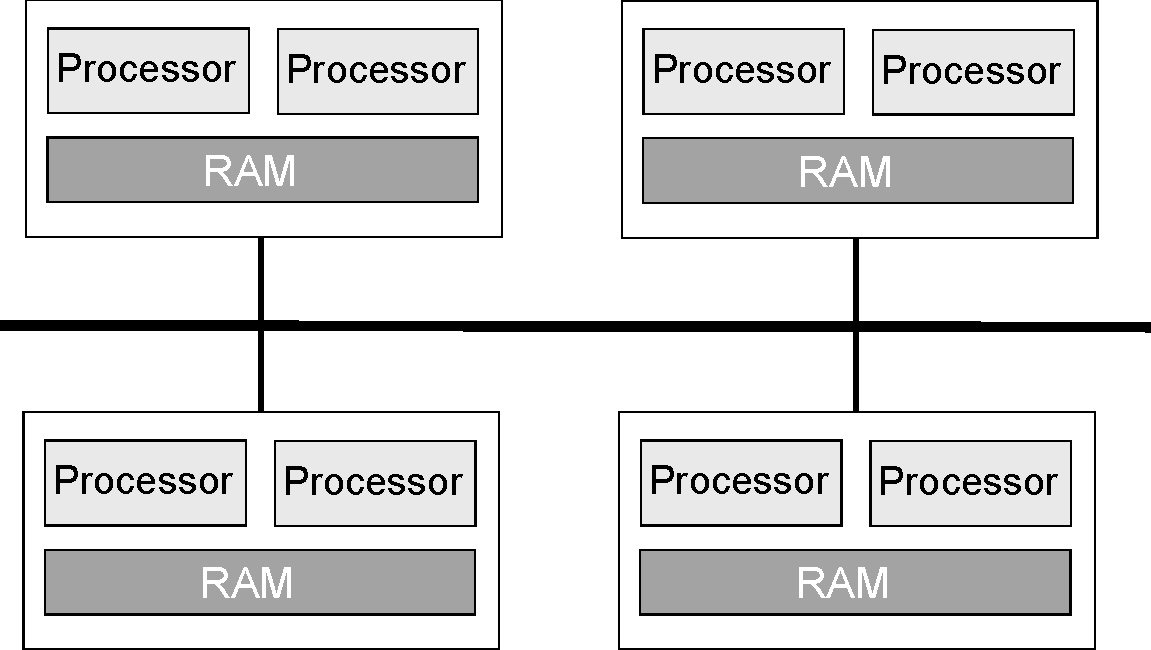
\includegraphics[width=0.48\linewidth]{cluster_cerfacs.pdf}
\label{fig:bull_nodes}}
  \caption{An example of a cluster: the Bull cluster at CERFACS\@. It consists of
  158 nodes (4 nodes are shown on \subcaptionref{fig:bull_nodes}). Each node has
  two Intel Sandy Bridge processors. One of them is shown on
  \subcaptionref{fig:bull_processor}.}
\label{fig:bull_cluster}
\end{figure}

\subsection{Programming models}
A program is `parallelized' by splitting the computation into independent tasks.
Each task is executed at the same time, between synchronizations. In practice,
parallelization can occur at several levels, depending on the
\textit{granularity} of the problem. Finding a properly granularity helps to
balance perfectly the computational load across all threads (\textit{load
balance}), an important goal in parallelization. With fine-grained tasks, it is
easier to achieve load balance but at the cost of \gls{overhead} due to
synchronization for example. On the other hand, coarse-grained tasks can decrease
the overhead by agglomerating small tasks into larger one. The granularity can
go from `instruction-level' parallelism to `thread-level' parallelism.
Considering the current architectures, we need to focus on `thread-level'
parallelism. Even so, finding the right granularity depends on the
application.
Some problems are `embarrassingly parallel', meaning parallelization is not an
issue. However, most application, in particular CTM models considered here, do
not fall into this category and require a programming paradigm. The two most
popular for cluster of processors are MPI and OpenMP\@.

\subsubsection{MPI}
\gls{MPI} is an \gls{API} for the message-passing paradigm. The
idea is to use `messages' for communication between processes in distributed
systems. MPI focuses on entities called \glspl{process}, with separate adress
spaces. MPI can also be used with multiple \glspl{thread}, but the two should
not be confused. The message-passing approach was already popular in the 1990s
and MPI was a standardization of different approaches. This contributed to its
popularity, along with its performance and scalability, even in shared-memory
environment.  It was not the only approach: \gls{PVM} was another solution but
has been supplanted by MPI in the 1990s. MPI is a standard and as such, has
several implementations (\textit{i.e}, the actual software): Intel MPI and Bull
MPI are vendor implementations, while OpenMPI and MPICH are open-source
implementations.

Each parallel task is assigned to a MPI process, which cannot access to data
from other processes. So blocks of memory (the `messages') are exchanged between
processes when needed. As explained below, these blocks do not necessarily need
to be contiguous. Here, we give more details for the different types of
communications used in Pangolin. Communications can take the form of
point-to-point communications, where a process A sends a message to another
process B. But global communications are also possible:
\begin{itemize}
  \item during a \textit{broadcast}, a process sends the same message to all
    processes,
  \item with a \textit{reduction}, a global operation is applied across all
    processes and the result is gathered onto a single process. For example, we can compute
    the global tracer mass across all processes,
  \item a \textit{barrier} synchronizes all processes at a given point
    in a parallel code.
\end{itemize}

An important aspect for a MPI process is to be able to avoid waiting for
communications --- \textit{i.e}, the arrival or departure of a message --- to end
before resuming its work. This is done using \textit{non-blocking}
communications. It should be noted than \textit{non-blocking} only means the
calling process can continue, not that communications are \textit{asynchronous}.
MPI has several non-blocking send modes but we will concentrate on
\texttt{MPI\_Isend}. Here, the sending process A sends to the target process
B a request for communication. While data is being transferred, A can continue
its computation, as long as it does not modify the data being sent. Once A has
received a confirmation from B, it can then reuse the data being sent. We only
mentioned here the relevant parts of MPI for Pangolin, but for more details
about MPI communications and MPI in general, the reader can refer
to~\cite{Gropp1999} for example.

One advantage of MPI is its portability: it can now be used on the majority, if not
all, of the current clusters of processors and can also run on desktops. It was
also designed for scalability in mind and works well up to hundred of thousands
of cores. However, future supercomputers aims for millions of cores
(\textit{exascale}) and MPI 1 and 2 have trouble scaling to these configurations,
mainly due to memory consumption, performance and fault tolerance, as explained
in~\cite{Thakur2010}. Another consideration when parallelizing a model is the
cost of implementation. Indeed, MPI requires rather important changes in the code
to be efficient and alternatives such as OpenMP may be attractive for a faster
development and incremental parallelization.

\subsubsection{OpenMP}
\gls{OpenMP} is an \gls{API} designed for shared-memory systems. Here, the model
used is the \textit{master-slave} model where a \textit{master} thread generates a set
of \textit{slaves} threads. Each one of them is assigned a task (either
statically or user-defined), then synchronized and terminated.  Like MPI, it is
very portable and works on most of shared-memory parallel architectures. Unlike
MPI, the cost of porting a code is much lower as OpenMP works by adding special
directives (the \texttt{pragma} keyword in C and \texttt{OMP} in Fortran) in the
sections to be parallelized. The most common operation is the parallel loop,
which allows for load balancing across threads and reduction operations for
example.
The downside to its ease-of-use is the lack of control of the programmer on data
layout, a possible limit to scalability. Nevertheless, its performances were
found to be better than MPI on shared-memory systems after optimizations. This
has led some applications to use hybrid programming by combining MPI
and OpenMP together. Examples can be found
in~\cite{Chorley2010,Jin2011,Guo2014}.

\subsection{Possible future trends}
Using flops as the unit measure, we are now in the \textit{petascale}
($10^{15}$) area and aiming for exascale ($10^{18}$ flops).
In~\cite{Perfect2004}, it was argued the current trends explained in the
introduction are going to continue: clock frequency will not increase, power
will be the primary constraint, flops will stay a cheap resource while data
movement will dominate. Furthermore, parallelism will
continue exponentially while memory will not scale according to the computing power.
\cite{Perfect2004} also argued that only hybrid architectures have a chance of
achieving exascale performance.

How does that impact us? In the case of Pangolin, advection is used as the
basis for parallelization with the MPI library. For that, a custom domain decomposition
technique is proposed in Section~\ref{subsec:domain_decompos}. It is a fairly
standard technique but communication \gls{overhead} becomes a concern when the
number of cores is too large for a given resolution. Also, the strategy chosen
here implies the different processes are equidistant, while in reality data
movement is more expensive outside the processor on clusters.  At the moment,
Pangolin does not have aim at such extreme configurations but focuses rather on
current clusters. This is why MPI was chosen, for both scalability and fine
control over parallelization.  Nevertheless, the warnings of~\cite{Perfect2004}
were heeded and some measures were taken to ensure the adaptability to the
future. First, we exploit as possible the algebraic features of the Pangolin
grid to reduce the memory cost of Pangolin.  This exploits the decreasing cost
of flops versus data movement. Another mitigation is to use hybrid programming
by combining OpenMP and MPI to use more cores than there are subdomains.

\label{subsubsec:paradigms}

\section{Parallelization strategy for the CTM}
\label{sec:strategy}
In a CTM, chemistry and advection are separate, independent tasks. Also,
advection of each tracer can be done independently of the others. However, this
granularity is not enough for a parallel model as the number of tasks would be
limited to the number of advected species (around a hundred). For large-scale
parallelization, it is best to focus on a domain decomposition technique, where
the computation domain is split into connex subdomains. Each parallel task is
then assigned a subdomain. As chemistry is local to each cell, only the
advection step requires communication between the subdomains so our
parallelization strategy focuses only on advection.

The computational load of advection is proportional to the number of
cells of a subdomain due to the Eulerian approach chosen here
(Section~\ref{sec:fv_schemes}). So the goal of the domain decomposition is to
create equal-area subdomains to achieve load balancing. We will first
focus on parallelizing the advection of one tracer. Multi-tracer advection will
simply aggregate the advection of the different tracers. We expect the
communication cost to be a linear function of the number of tracers.  The
underlying hypothesis is that the cost of chemistry is constant for all cells.
It is not the case in practice, due to factors such as cloud or the day-night
interface. Nevertheless, mitigation for load unbalancing do the chemistry is
studied in Section~\ref{sec:future_work}. For the advantages mentioned before
(scalability, fine control, portability), we have chosen to use MPI as the
parallel library and paradigm. The code itself is written in Fortran.

\subsection{Domain decomposition}
\label{subsec:domain_decompos}
It should be noted our strategy should not be confused with `classical' domain
decompositions techniques, where boundary conditions are searched algebraically.
Here, we aim at splitting our custom quasi-area preserving grid into equal-sized
subdomains for the advection scheme. As mesh splitting is a common issue,
professional tools are available, such as Scotch (\cite{Pellegrini2012}) or
Metis (\cite{Karypis1995}). These tools use graph algorithms to create
high-quality partitionings. However, such methods are generic and do not take
into account the specific structure of the Pangolin grid and this leads to
unstructured subdomains as shown on Fig.~\ref{fig:scotch_54}. As such, it discards
the algebraic features of the grid, such as the computation of neighbors cells.
We have chosen instead to develop our own partitioning to exploit these algebraic
features. The main consequence is that information is recomputed as much as
possible, instead of being stored in memory. For example, the neighbours of a
cell (given by Eq.~\eqref{eqn:neighb_merid}) and the neighbours of a subdomain (see below)
are computed when needed. This follows the trend mentioned before, where flops
are cheap versus data movement. We explain here how the partitioning is
performed.

We have seen the Pangolin grid has four axes of symmetry, creating six identical
zones (Fig.~\ref{fig:pango_zones}). First, we focus on splitting one zone.  As
it contains exactly $N_{lat}^2$ cells, the optimal number of subdomains is of
the form $p^2$, with $p$ dividing $N_{lat}$. In this case, all subdomains on a
zone have exactly the same area (${(N_{lat}/p)}^2$ cells).  There are several
possibilities for the topology of the $p^2$ subdomains. The most natural
configuration for the subdomains is to use the same topology as the grid itself.
On zone 1, subdomains are set on bands, where the $i$-th band contains $2i-1$
subdomains.  This topology can be extended to the whole grid if the total number
of subdomains is $6p^2$, with $p$ still dividing $N_{lat}$: the subdomains are
placed on each zone according to the algorithm mentioned before. The topology on the
Southern hemisphere is simply symmetric in respect to the Equator.  This results
in the global decomposition on Fig.~\ref{fig:pangolin_54}. In this optimal
configuration, computing the neighbours of a subdomain and the interface between
two subdomains is easy. It also helps reducing the number of neighbours of a
subdomain (see below for a more detailed comparison with Scotch). It should be
noted that the FARSIGHT transport scheme by~\cite{White2011} (presented in the
testing suite in Section~\ref{sec:comparison}) has a similar constraint on the number
of subdomains. The constraint comes from the cubic grid: each face has a square
number of cells so the total number of the subdomains should be of the form
$6p^2$.  To ensure each face of the cube has $p$ subdomains of equal area, $p$
has to be a divisor of the number of cells along an edge.

In order to relax the requirement on the number of subdomains (\textit{i.e}, the
number of cores), let us focus again on partitioning only one zone. If the
number of subdomains $p'$ is not a square, we find the closest best match
$q=\lfloor \sqrt{p'}\rfloor$. Then we can apply the algorithm described before
to place the $q$ subdomains. The remaining $p'-q$ subdomains are then placed on the
last band --- \textit{i.e}, the one closest to the Equator. It should be noted
that $q$ does not need to divide $N_{lat}$. In this case, the `height' of
the last band will be changed to include the remainder of the division.  On the
last band, subdomains have a much smaller size than the other $q$
domains. They are set in the following way: the first $p'-q-1$ subdomains
are rectangular and of equal size, while the last one is trapezoidal with more
cells. If the last band is too thin, other bands are slightly reduced to
increase the height of the last band. The same strategy is applied to the other
five zones to provide a global decomposition. Thus the only constraint is the
total number of subdomains is a multiple of $6$. An example of this global
partitioning is presented on~Fig.~\ref{fig:pangolin_72}.\\
We can still go a bit further into relaxing the constraint on the number of
domains. So far, the same strategy was applied for each zone. Instead, the final
version of our partitioning only requires the total number of subdomains to be of
the form $3p$. This is done by only requiring that zones 1, 2, 3 and 4, 5, 6 have
each the same number of subdomains, but the number of subdomains could be different on
each hemisphere.

Where does that leave us? Our partitioning works best in some optimal
configurations, \textit{i.e}, when the total number of subdomains is $6p^2$ with
$p$ dividing $N_{lat}$. For more flexibility on the number of cores, this
condition can be relaxed to a number of subdomains of the form $3p$. However, the
limiting factor for speed-up (defined more precisely in
Section~\ref{sec:performances}) is the size of the largest subdomains, which only
changes for optimal configurations. In practice, it means that adding more cores
between optimal configurations will not improve the performances. Nevertheless,
this provides a flexibility which can be used later for improving load-balancing
of the chemistry for example, or for allowing a different number of threads in a
hybrid MPI-OpenMP configuration.

\subsubsection{Comparing the partitioning by Scotch and Pangolin}

Here we examine in more details the difference between our algebraic
partitioning and a general-purpose mesh partitioner, Scotch. For a visual
comparison, Fig~\ref{fig:54_domains} shows the partitioning by Scotch and
Pangolin in a optimal case for Pangolin, while Fig~\ref{fig:72_domains} shows
the partitioning in a sub-optimal case for Pangolin. It is immediately apparent
there is no underlying structure in the partitioning computed by Scotch. From a
performance point of view, it means that both the topology of the subdomains and
the interface size between subdomains need to be represented using a custom data
structure. As it increases the memory storage, it conflicts with the possible
future trends mentioned before and should be avoided.

The quality of the partitioning is quantified more precisely in
Table~\ref{tab:scotch_compare}. Subdomain size is roughly the same for both Scotch
and Pangolin in the optimal case for Pangolin. For a suboptimal number of
domains, load-balancing is less interesting as can be expected. However, the
total number of neighbours is more beneficial for Pangolin: the subdomains created
by Scotch have in average $2.5$ more neighbours, even in the suboptimal case.
This makes our partitioning more interesting as it requires a lower number of
neighbours.  It will decrease accordingly the number and volume of
communications. From a computational point-of-view, the neighbours of a subdomain
are computing using only integer arithmetic. While there are special cases when
the number of subdomains is sub-optimal, computation still remains extremely cheap.
When searching for the interface between two subdomains, the idea is to find the
intersection between the extremities of the subdomains and the neighbours cells of
the adjacent subdomain.  Again, this is mostly integer arithmetic, along with some
floating-point computations. Therefore, we exploited as much as possible the
algebraic features of the Pangolin grid to use the cheaper cost of flops versus
data storage.

\begin{figure}
  \subbottom[Pangolin]{%
    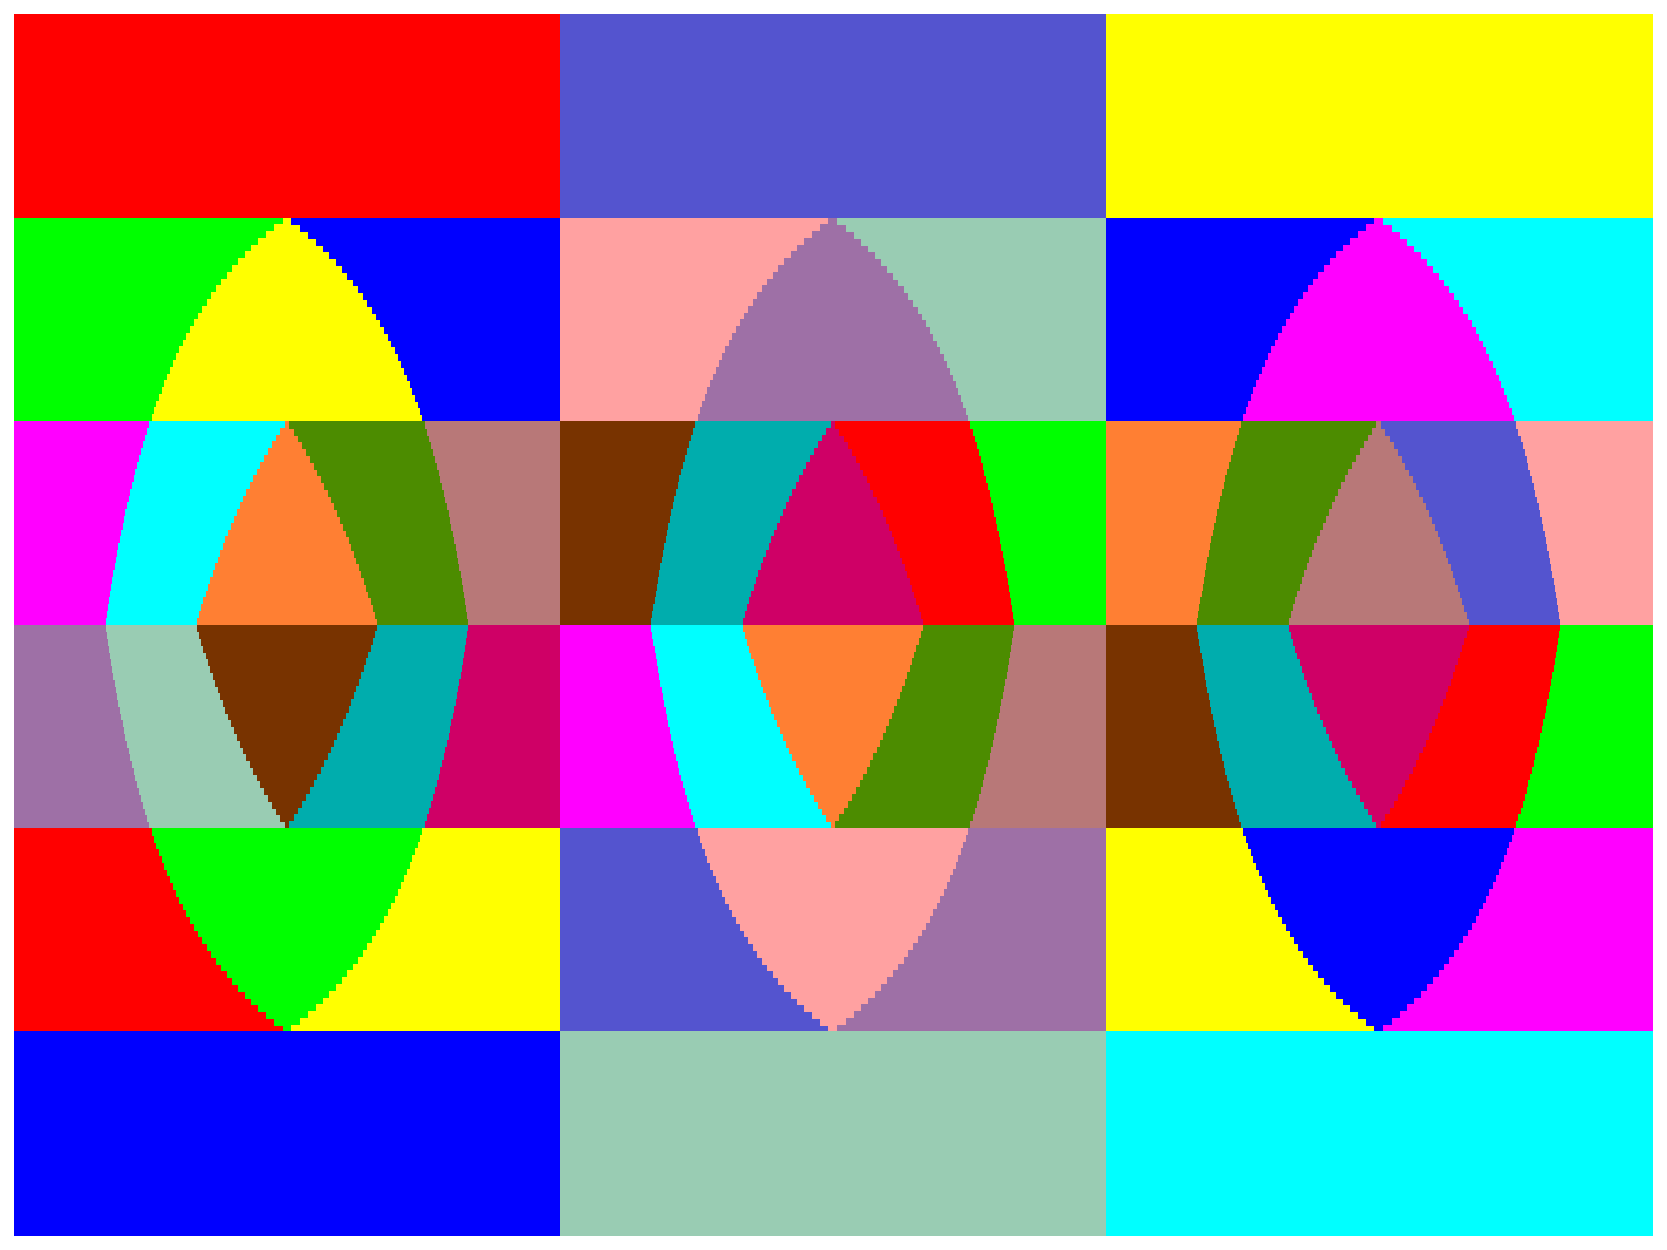
\includegraphics[height=5cm]{partitioning_54.pdf}
\label{fig:pangolin_54}}
  \hfill
  \subbottom[Scotch]{%
    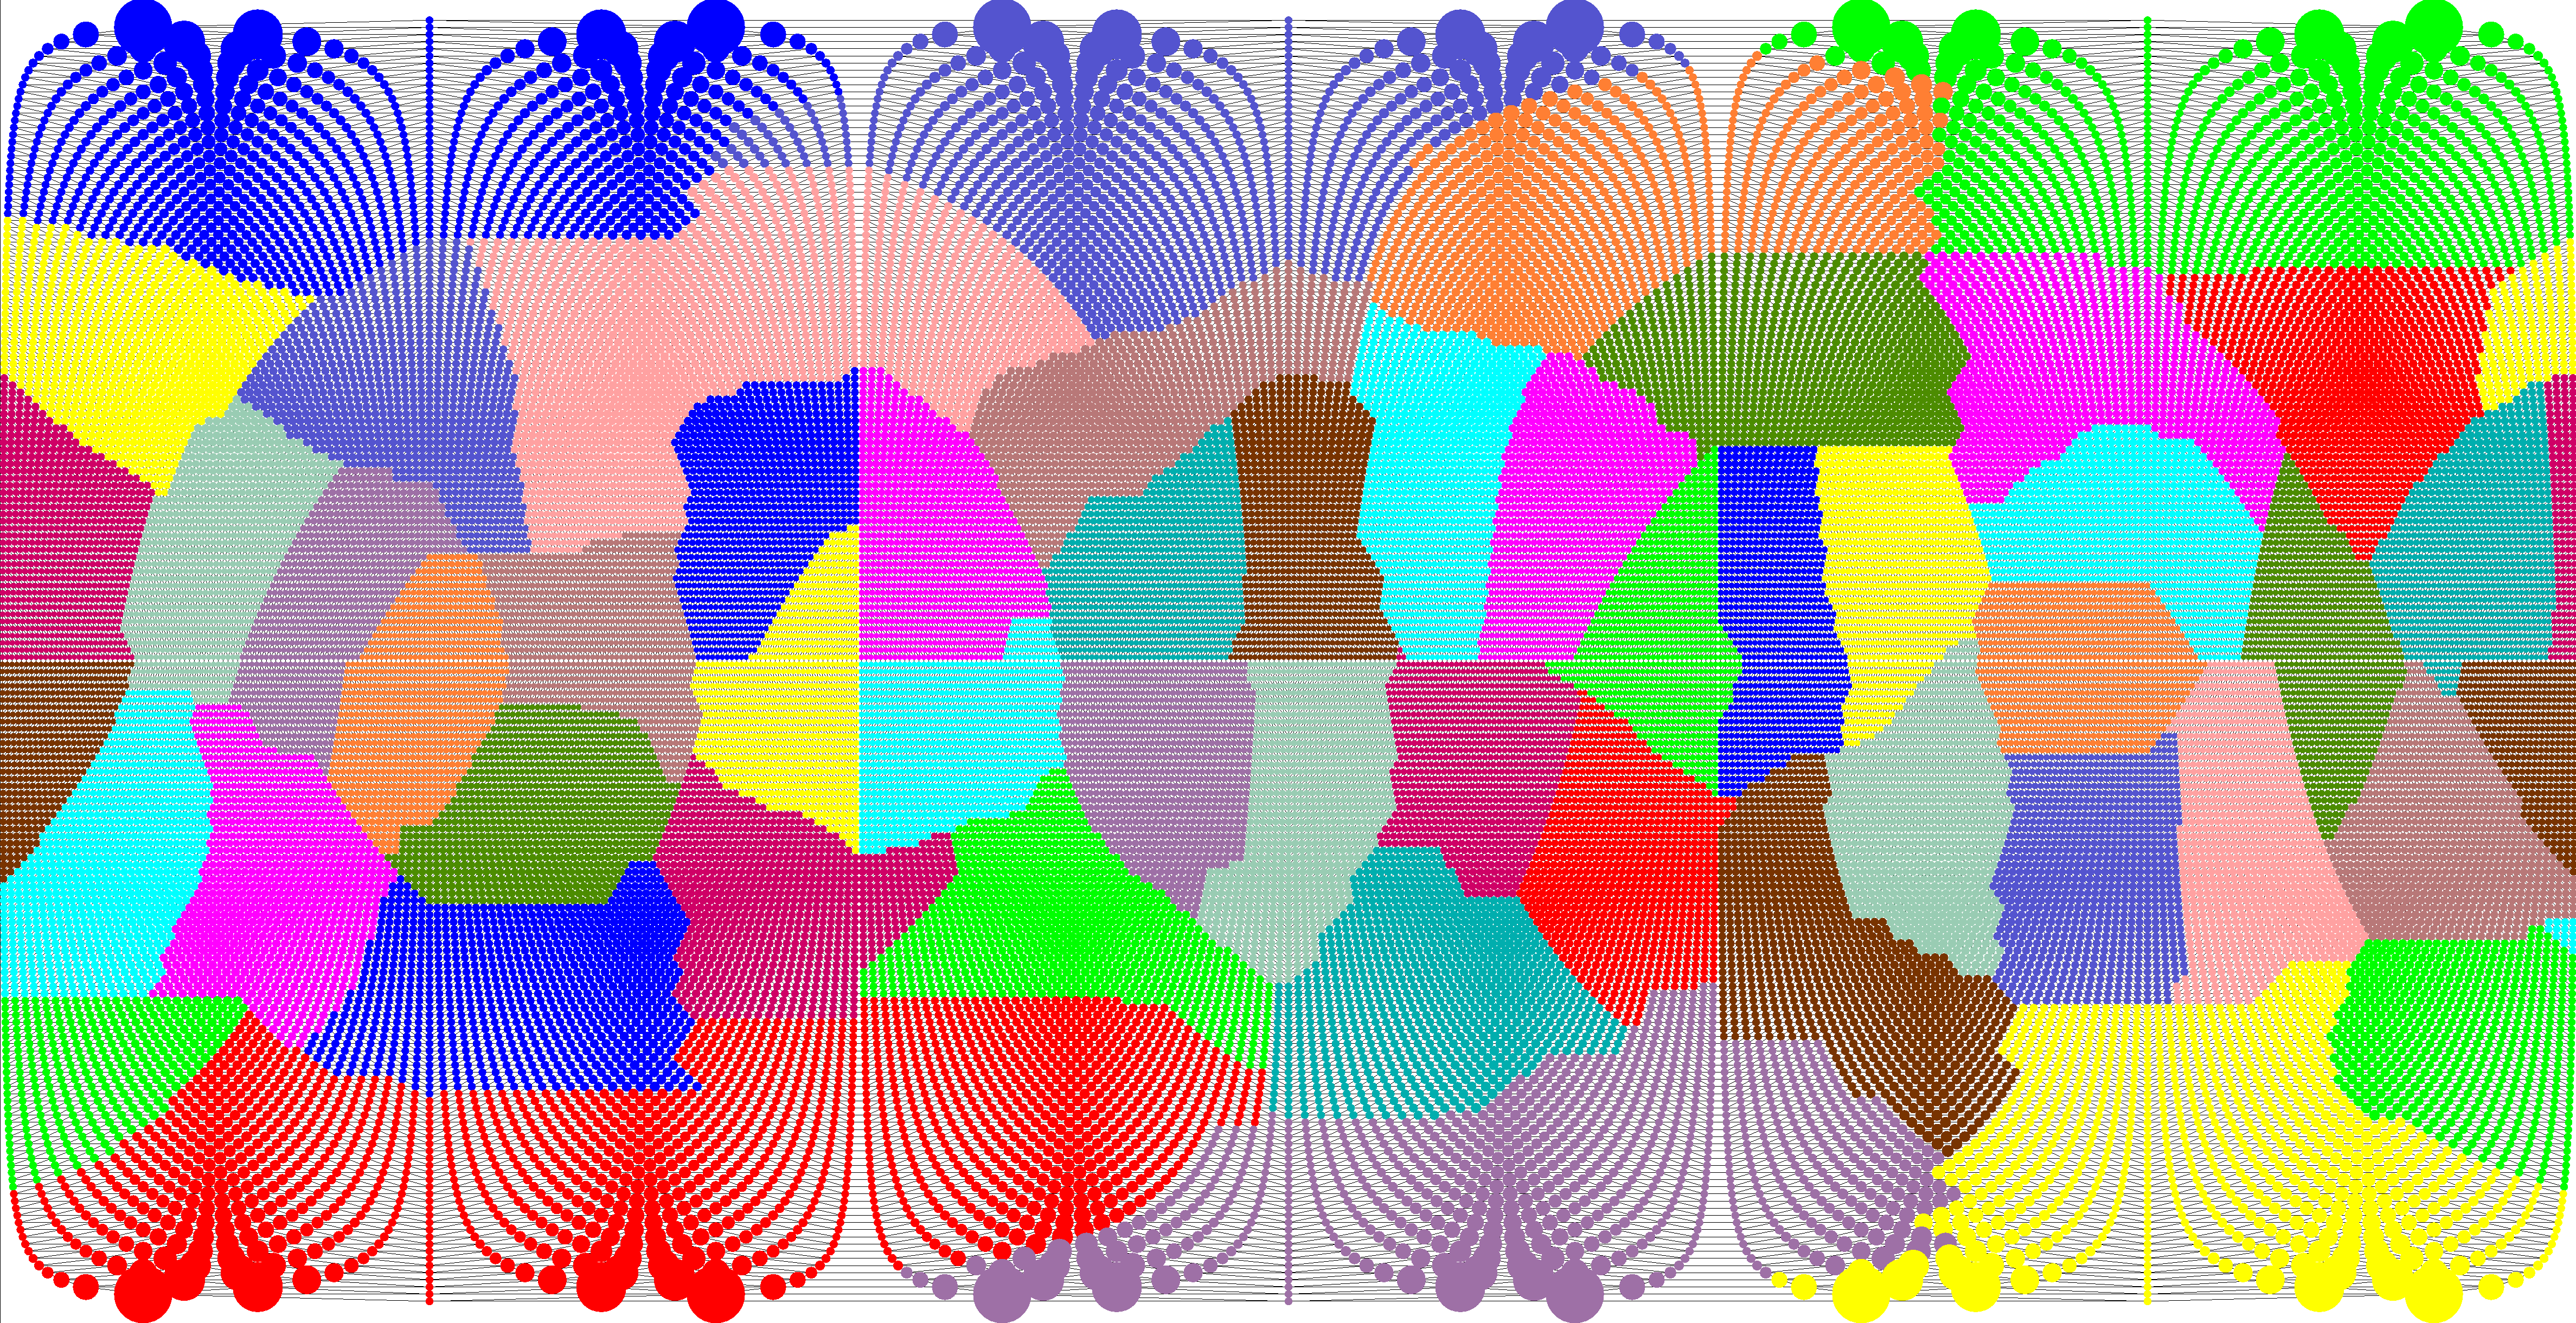
\includegraphics[height=5cm, width=0.5\linewidth]{scotch_54cores.png}
\label{fig:scotch_54}}
  \caption{%
    Comparison of our algebraic partitioning
    \subcaptionref{fig:pangolin_54} to Scotch \subcaptionref{fig:scotch_54} for 54 subdomains
    (optimal case for Pangolin).  Each color corresponds to a subdomain (the
    same color can be used for different subdomains). The total number of
    cells is 8100. Grids are shown in latitude-longitude coordinates.
  }
\label{fig:54_domains}
\end{figure}

\begin{figure}
  \subbottom[Pangolin]{%
    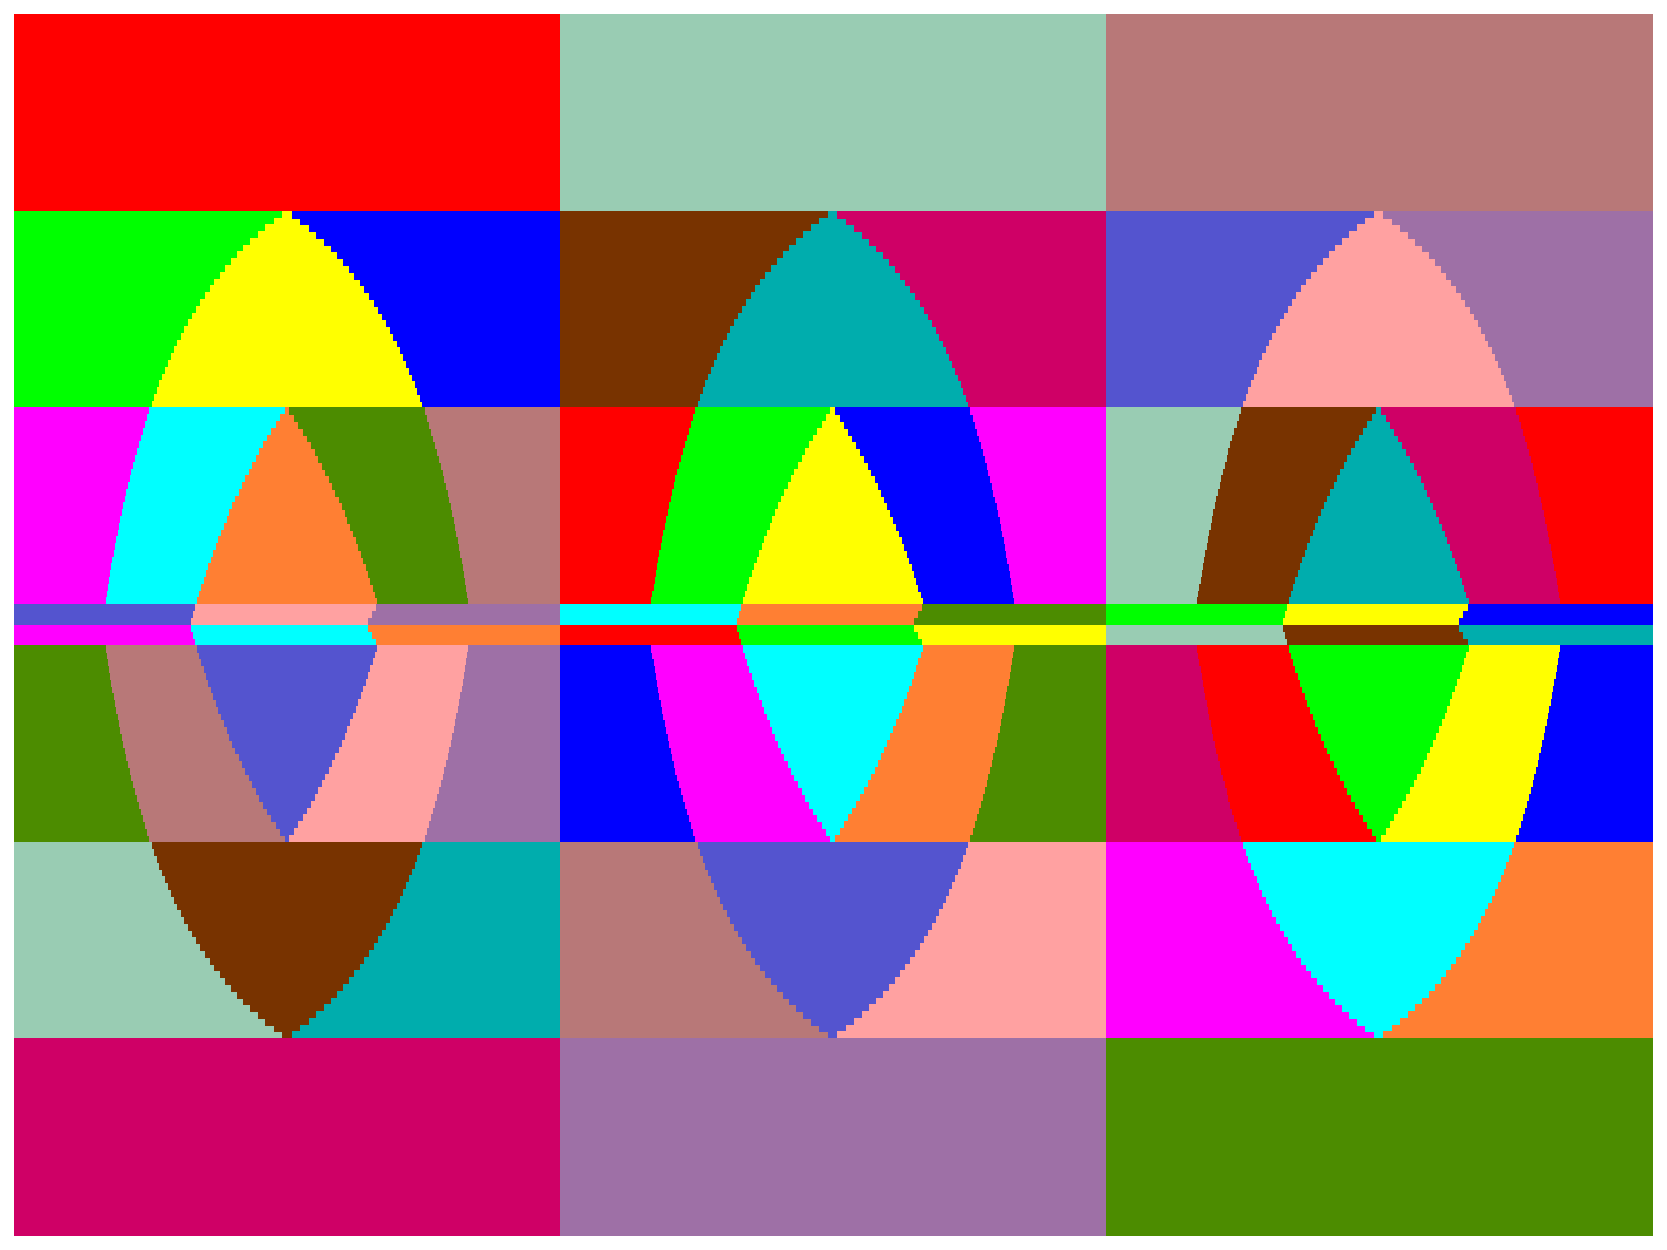
\includegraphics[height=5cm]{partitioning_72.pdf}
\label{fig:pangolin_72}}
  \hfill
  \subbottom[Scotch]{%
    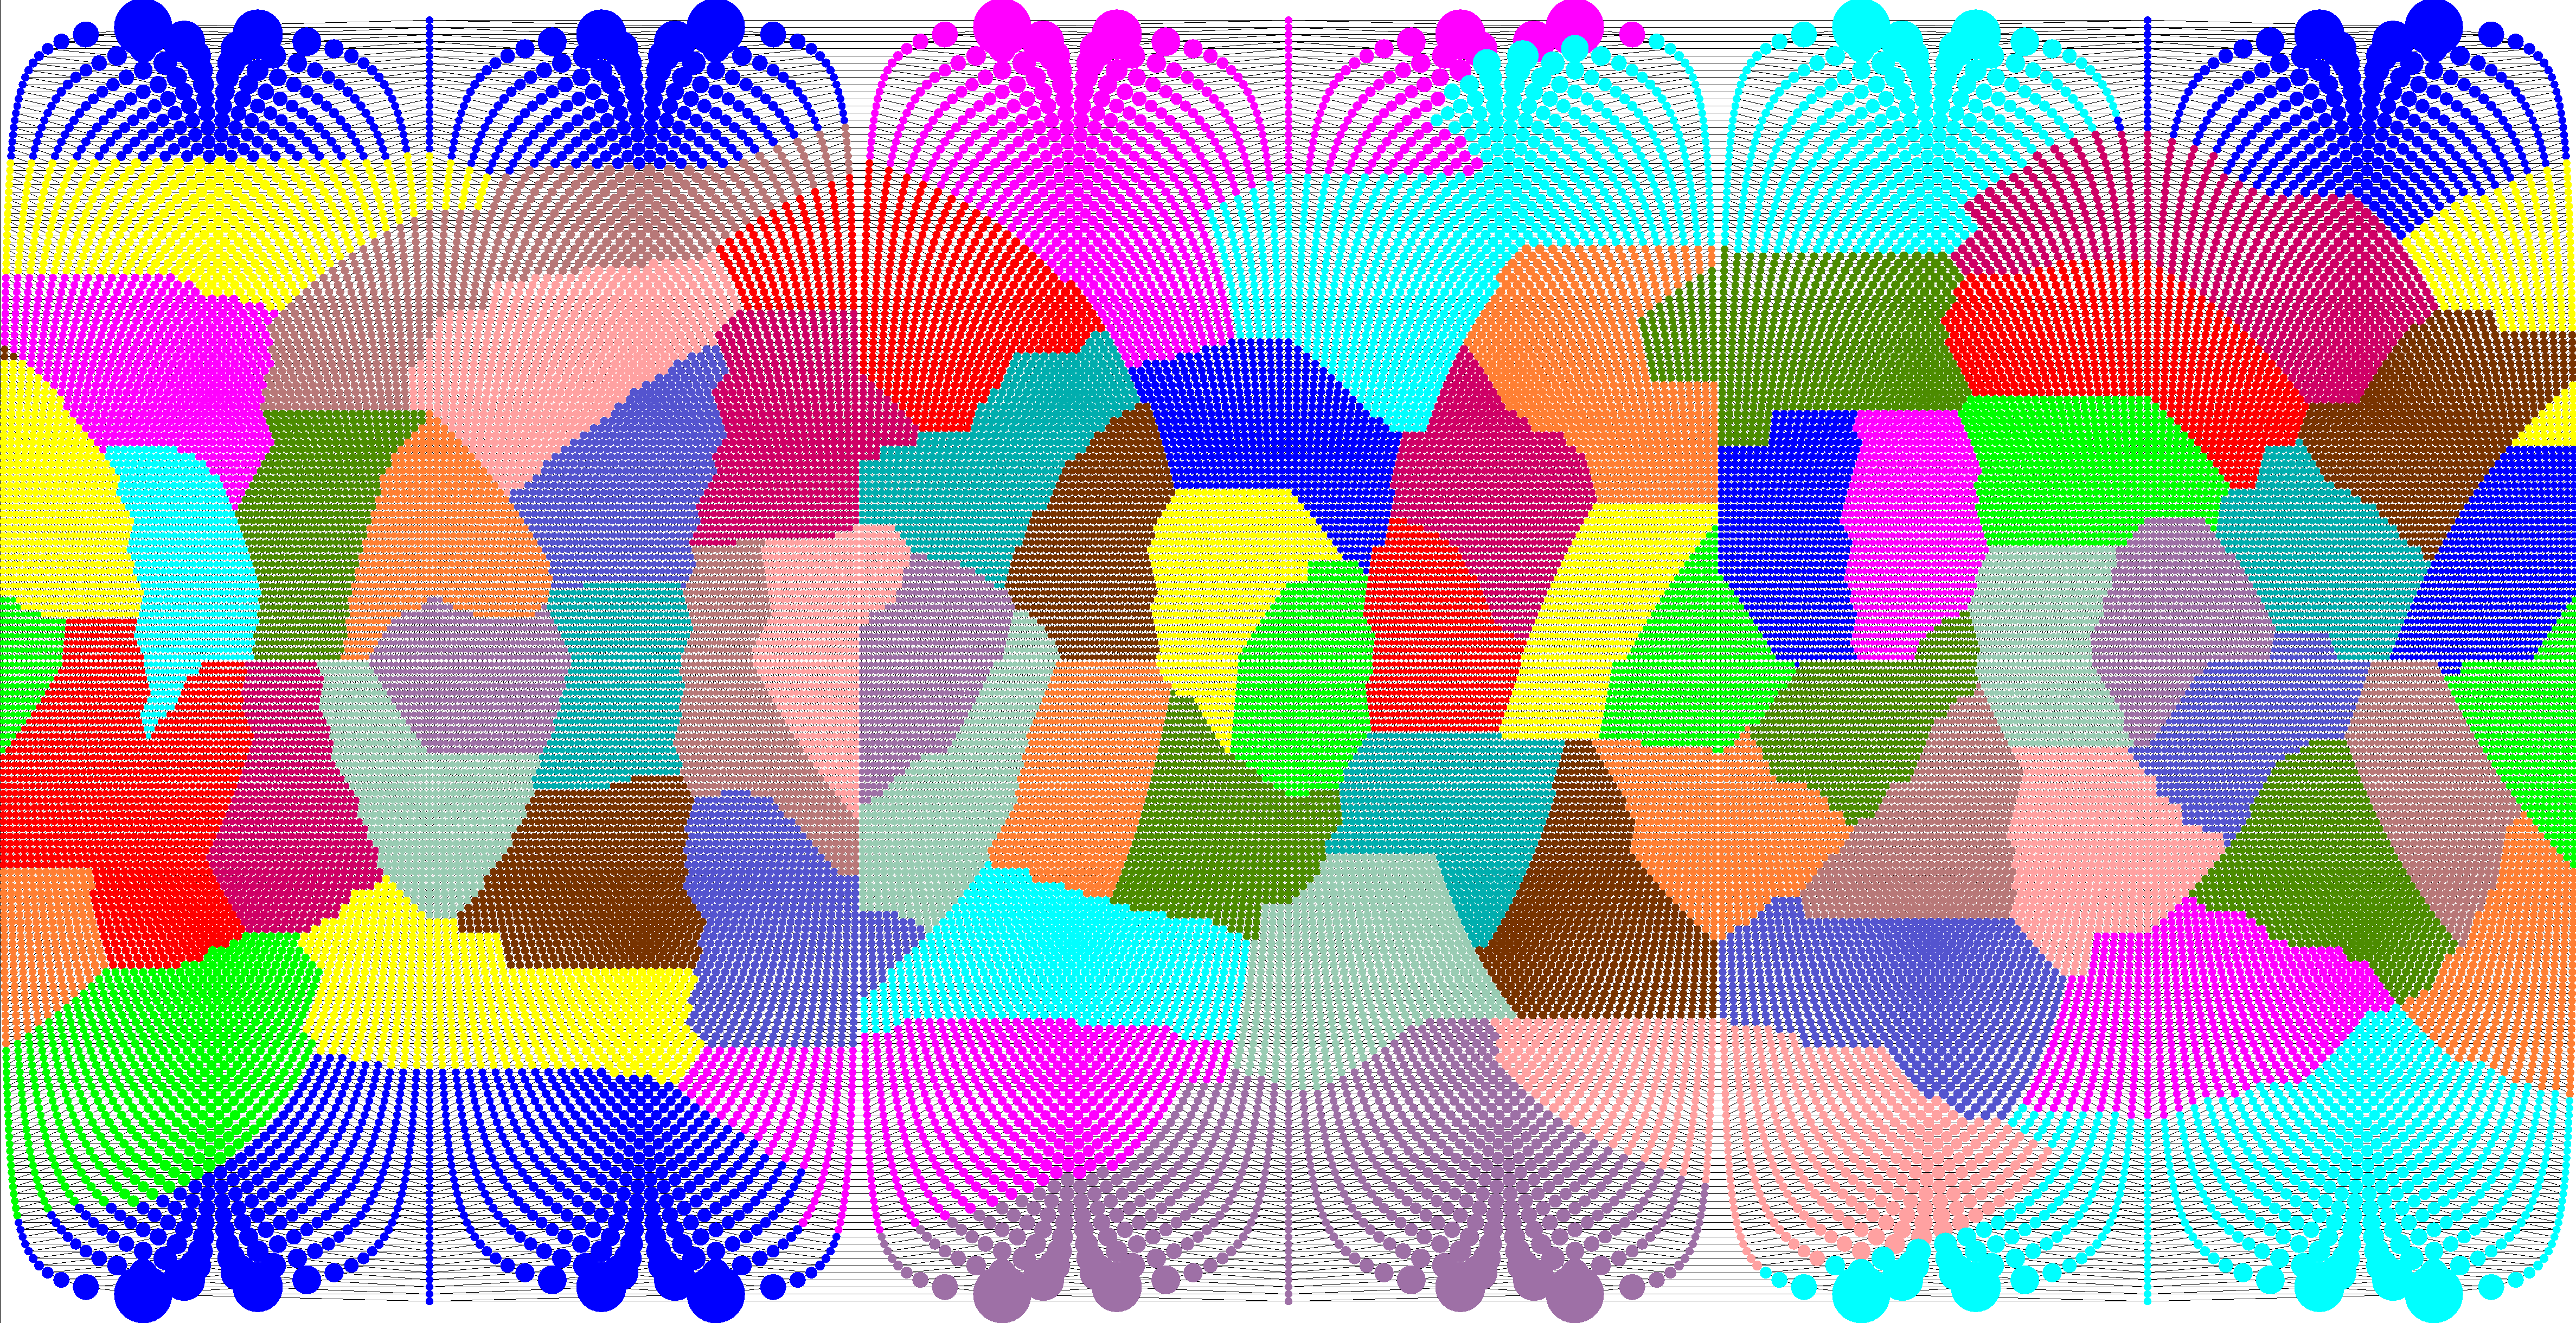
\includegraphics[height=5cm, width=0.5\linewidth]{scotch_72cores.png}
\label{fig:scotch_72}}
  \caption{%
    Comparison of our algebraic partitioning
    \subcaptionref{fig:pangolin_72} to the general purpose mesh
    partitioner Scotch \subcaptionref{fig:scotch_72} for 72 subdomains
    (optimal case for Pangolin).  Each color corresponds to a subdomain (the
    same color can be used for different subdomains). The total number of
    cells is 8100. Grids are shown in latitude-longitude coordinates.
  }
\label{fig:72_domains}
\end{figure}

\begin{table}
 \centering
  \begin{tabular}{*{7}{c}}
    \toprule
    & \multicolumn{3}{c}{Domain size} & \multicolumn{3}{c}{Neighbours} \\
     \cmidrule(r){2-7}
    & min & max & avg & min & max & sum \\
     \midrule
    Scotch 54 cores & 899 & 901 & 900 & 3   & 8   & 304\\
    Pangolin 54 cores & 900 & 900 & 900 & 3   & 6   & 123 \\
     \midrule
    Scotch  72 cores & 661 & 689 & 675 & 3   & 9   & 416\\
    Pangolin 72 cores & 174 & 841 & 675 & 4   & 6   & 159 \\
    \bottomrule
  \end{tabular}
  \caption{Comparaison of the quality of the partitioning by Scotch and Pangolin
  (54 and 72 subdomains respectively). A dual recursive
    bipartitioning was used for Scotch.}
\label{tab:scotch_compare}
\end{table}

\paragraph{Grid generation}
As mentioned in Section~\ref{subsubsec:description}, the Pangolin grid is
completely defined by the number of latitudes $N_{lat}$ on an hemisphere and the
number of cells at the poles. So the cost of storage of the global grid is
virtually free, which is a huge advantage over unstructured grids.  Another
advantage of our algebraic partitioning is to preserve this lightweight
structure even after the decomposition. Knowing the number of `bands' on
a zone, we can deduce the shape of the subdomain has a square number of cells or
not and then deduce the shape of the subdomain (squared/triangular on normal
bands or rectangular/trapezoidal on the last band). In the end, a subdomain is
simply defined by two integers: the band number and the position in this band.
This is extremely advantageous as the cost of storing subdomain is virtually
free, especially when compared to unstructured domains, which must store the
cell connectivity as well as the coordinates for all cells of each subdomain. 

\subsection{Advection algorithm}
\label{subsec:parallel_advection}
In flux-form finite volume advection schemes, the tracer ratio in a cell is
updated according to fluxes at the borders (Section~\ref{sec:fv_schemes}). In
1D, the air and tracer mass are updated according to Eq.~\ref{eqn:air_update}
and~\ref{eqn:air_update}, with the tracer fluxes defined by
Eq.~\eqref{eqn:vanleer1} and Eq.~\eqref{eqn:slope}. 2D transport is achieved by
applying 1D advection operators successively. From a parallelization point of
view, the synchronization points are:
\begin{itemize}
  \item after computing the 1D gradient,
  \item after computing the 1D fluxes,
  \item after updating the tracer ratios.
\end{itemize}
In a message-passing context, data outside the current subdomain is not available.
As the advection scheme require some information outside the current subdomain, a layer of
additional cells, called \textit{ghost cells}, is created around the subdomain. Data from neighbouring subdomains
will then be copied into these ghost cells. Their layout is illustrated
on Fig.~\ref{fig:ghost_cells}. The number of layers of ghost cells depends on
the stencil of the scheme used. For the van Leer scheme chosen here, only one
layer of ghost cells is needed.

To parallelize each step, the same strategy is used: first, we post a request
for non-blocking communications. While communications are taking place,
computations are performed at the \textit{interior} of the grid, \textit{i.e},
where no data outside the current subdomain is needed. Then we check if the
communications are finished and resume computation, this time at the
\textit{border} of the grid, \textit{i.e}, where data outside the subdomain is
needed. Non-blocking communications should be able to `hide' the communications
cost (message transfer and throughput) so that no time is lost waiting for data
to be exchanged. Of course, this supposes the communications
complete faster than the computation on the interior. Once the subdomains become
small enough, this is no longer true so time will be wasted by waiting for
communications to complete.
The resulting algorithm for zonal advection is rather straightforward and is
presented in Algorithm~\ref{algo:zonal}. An extra step must be added for the
meridional transport: due to semi-structured of the grid, computing the
meridional gradient requires an interpolation as shown on
Fig.~\ref{fig:merid_interpol}. The resulting algorithm is shown on
Algorithm~\ref{algo:merid}.
\begin{algorithm}
  \caption{Parallel 1D zonal advection}
\label{algo:zonal}
  \begin{algorithmic}
    \Require All tasks are synchronized
    \Ensure Ratios are updated with new values from 1D zonal advection
    \State Starts the communications for ratio in ghost cells 
    \State Compute the zonal gradients on the interior
    \State Wait for the end of communications
    \State Compute the zonal gradients on the boundary
    \State
    \State Starts the communications for zonal gradient in ghost cells
    \State Compute the zonal fluxes on the interior
    \State Wait for the end of communications
    \State Compute the zonal fluxes on the boundary
    \State
    \State Update the boundary and interior ratios
  \end{algorithmic}
\end{algorithm}

\begin{algorithm}  
  \caption{Parallel 1D meridional advection}
\label{algo:merid}
  \begin{algorithmic}
    \Require All tasks are synchronized
    \Ensure Ratios are updated with new values from 1D meridional advection
    \State Starts communications for ratio in ghost cells 
    \State Compute zonal gradient on the interior
    \State Wait for end of communications
    \State Compute zonal gradient on the boundary
    \State
    \State Starts communications for zonal gradient in ghost cells
    \State Compute meridional gradient on the interior
    \State Wait for end of communications
    \State Compute meridional gradient on the boundary
    \State
    \State Starts communications for meridional gradient in ghost cells
    \State Compute meridional fluxes on the interior
    \State Wait for end of communications
    \State Compute meridional fluxes on the boundary
    \State
    \State Update boundary and interior ratios
  \end{algorithmic}
\end{algorithm}

Due to the structure of the Pangolin grid, ghost, border
and interior cells have different shape and size for zonal and meridional advection, as shown on
Fig~\ref{fig:ghost_cells}. For zonal advection, a subdomain only needs to
communicate with its east and west neighbours, while it requires communications
with all of its neighbours for meridional advection. Inside a subdomain, the
neighbours of a cells are also different in the zonal and meridional case: a
cell has more than two meridional neighbours but has only two zonal neighbours.
Also, meridional interpolation requires to have also the east and west cell
neighbours, in addition to the north and south neighbours. This explains the
`stair-like' structure for meridional boundary cells. We can draw several
conclusions from that. First, most of the computation occurs during the meridional step. Second, meridional
advection needs twice the communication volume of zonal advection. Finally,
meridional advection is also the most restrictive operation if communications
are to be `hidden' as the ratio number of cells over ghost cells is less
favorable than in the zonal case. These differences are highlighted in
Table~\ref{tab:size_interior}, which shows the exact ratio between ghost, interior and
border cells to the total number of cells (outside ghost cells).

\begin{figure}
  \begin{minipage}{0.49\linewidth}
    \includegraphics[width=\linewidth]{ghost_cells_we.pdf}
  \end{minipage}
  \begin{minipage}{0.49\linewidth}
    \includegraphics[width=\linewidth]{ghost_cells_ns.pdf}
  \end{minipage}
  \caption{%
    Ghost, boundary and interior cells for zonal (left) and meridional
  (right) advection for a rectangular subdomain.}
\label{fig:ghost_cells}
\end{figure}

\begin{table}
 \centering
 \begin{tabular}{ccc}
    \toprule
    & Zonal & Meridional \\
     \midrule
     Ghost & $2/n$ & $(4n+1)/n^2$\\
     Border & $2/n$ & $(4n-1)/n^2$ \\
     Interior & $(n-1)/n$ & ${(n-2)}^2/n^2$ \\
    \bottomrule
  \end{tabular}
  \caption{Comparison of the size of ghost, border and interior cells for zonal
  and meridional advection. A subdomain of $n\times n$ cells is considered here and
  ghost cells are not counted.}
\label{tab:size_interior}
\end{table}

\paragraph{Custom MPI communications}
As mentioned before, we exploit the features of \gls{MPI} to hide 
communication costs with non-blocking communications. Fortunately, we do not have
to send contiguous blocks of data by hand as MPI provides user-defined
datatypes. As Pangolin has a semi-structured grid, data is stored as an 1D array.
Therefore, defining datatypes adapted to ghost cells for example means the
indexed structure must be used (\texttt{MPI\_Type\_indexed}). It defines 
irregularly-spaced block of data, where the blocks can be of different
lengths.
Two examples on how the datatypes are constructed are shown on
Fig.~\ref{fig:datatypes}. For each neighbour of a subdomain, two datatypes must be
defined: one for ghost cells --- receiving data from the neighbour --- and one
for interior cells --- sending data to the neighbour. Of course, these are not
the only datypes offered by MPI but it fits our data structure well.  To create
higher-level datatypes for more readable communications, we used the
\textit{struct} datatype (\texttt{MPI\_Type\_create\_struct}) in Pangolin.

Now that we know what data to communicate, let us examine the communication
protocol. As a reference, the different send modes of MPI are shown in
Appendix~\ref{app:mpi_send}. From the performance tests (see 
Section.~\ref{sec:performances}), non-blocking communications works best with
\texttt{MPI\_Isend} on our cluster, matched with a \texttt{MPI\_Irecv}. As data
being send to (or received from) is directly read from (or written to) the
actual data in memory, data in the border cells cannot be over-written before the
transfer have been completed. After the computation is performed on the interior
cells, we check if all requests have been completed with \texttt{MPI\_Waitall}.

\begin{figure}
  \subbottom[Interior cells for the east neighbour of the
  subdomain (in red).]{%
    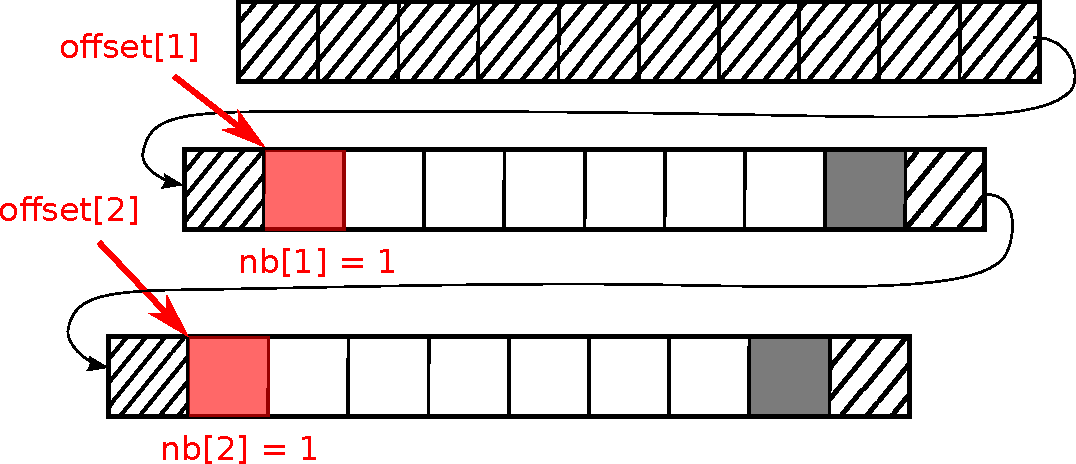
\includegraphics[width=0.48\linewidth]{zonal_border.pdf}
\label{fig:zonal_border}}
  \hfill
  \subbottom[Interior cells for the two northern neighbour of the
  current subdomain (in red and blue).]{%
    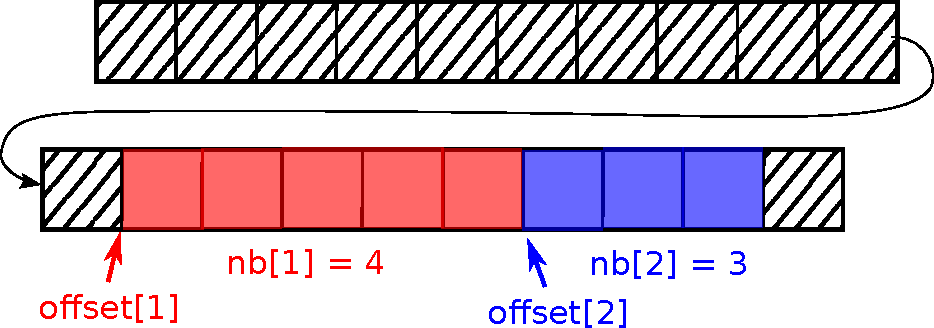
\includegraphics[width=0.48\linewidth]{merid_border.pdf}
\label{fig:merid_border}}
  \caption{Examples of two MPI derived datatypes for interior cells using the
    \textit{indexed} structure. Datatypes are constructed as a set of blocks, where
    each block is defined by an \texttt{offset} and a size (\texttt{nb}) array. Data
    is a contiguous 1D array in memory. Ghost, border and interior cells are
  shown as hatched, filled and empty cells respectively.}
\label{fig:datatypes}
\end{figure}

\paragraph{Multiple tracers}
Advecting multiple tracers is done by simply repeating the advection of a single
tracer for each tracer. To decrease communication costs, all tracer data is sent at once, instead of sending a message for each tracer. From the
point of view of MPI, once a datatype has been created for a tracer, the
datatype for all tracers is simply the union of these single-tracer datatypes.
It is expected performance will scale linearly according to the number of tracers (see
Section~\ref{subsec:results}) as the latency penalty only needs to be paid once
for all tracers.

\section{Input/Output}
Due to the increase of computational power, CTMs have been using finer and finer
resolutions, thus managing larger and larger datasets. On top of that, CTMs need
to read and write data periodically and efficiently in operational contexts. I/O
can no longer be done sequentially and need to exploit parallelism. Here we
examine the different alternatives in the context of parallel I/O.  The first
strategy is that each process writes its own data on a separate file. It has the
advantage of being rather easy to implement. Yet it makes post-processing
difficult, as the global structure (shape and position) of the process is lost
after the simulation, especially for Pangolin. Another disadvantage is that
restarting the simulation with a different number of cores requires an extra step
to interpolate data to the proper number of files. A second approach is to
reserve a process for I/O only, which will receive and send data to or from
other processes. A third solution is that all processes write to the same file,
using either custom functions or high-levels libraries. 

Unfortunately, there is neither an unique solution, nor a perfect implementation
for all problems. A solution would be to skip I/O entirely for periodic output
and run the simulation again when the data is needed. This approach only works
when the computation is less expensive than data storage. In the case of CTMs,
it is not an option as periodic read must occur. Either way, performance is
attained by benchmarking the different alternatives and tuning one of them to
the problem at hand for the available hardware. We now explain the evolution of
I/O in Pangolin, from a sequential model to a fully parallel version.

\subsection{Sequential}
In our first version, each process wrote in turn in the same file. Using MPI,
the processes passed around a \textit{token}, which allowed the current holder
to write in the file. This can be seen as a distributed implementation of a lock.
The algorithm to read/write for a subdomain is highlighted in
Algorithm~\ref{algo:io_seq}. The idea is to read/write all cells until we
are in the desired subdomain.
The output format is ASCII, a human-readable format. Unfortunately, it does not
provide compression, a highly desirable feature for large datasets. Using binary files would
be a solution to reduce the size of the dataset but would require to implement
our own I/O strategies. We have chosen to use a parallel I/O library to
parallelize our sequential algorithm. Three of them are presented below.

\begin{algorithm}
  \caption{Sequential ASCII read/write}
\label{algo:io_seq}
  \begin{algorithmic}
    \Require The current process has the token
    \Ensure Domain data is read from/written to file and token is passed on
    \State Skip all latitude lines up to $first\_line$
    \For{$i=first\_line, last\_line$}
      \For{$j=1, \text{nb\_cells}(i)$}
        \If{$(i,j)$ is in the subdomain}
          \State Read/write cell $(i,j)$
        \EndIf
      \EndFor
    \EndFor
    \State Rewind file
    \State Pass token to the next process
  \end{algorithmic}
\end{algorithm}

\subsection{Parallel}
\paragraph{MPI-IO}
One solution to read or write in parallel a shared file is the MPI-IO
library (a recent description is given in~\cite{Liao2014}). It was defined in
the MPI 2 standard and as such is a natural choice for a MPI application.
However, it is a rather mid-level approach and is used in practice by
higher-level libraries. It can also create some portability issues due to
low-level specifications such as \gls{endianness}.

\paragraph{netCDF}
While there is no standard file format for in climate or weather community,
\gls{netCDF} is the format which comes closest to that. It is a high-level
library with its own portable format, providing parallelism in two ways. Native
parallelism is available with the Parallel netCDF (\cite{Li2003}) or, starting
with netCDF 4, using the parallelism of HDF5 shipped with it. Unfortunately, it
is targeted at the regular latitude-longitude grid and does not support 
unstructured grids well. In Pangolin, we would like to define custom regions in our
grid to read or write directly to/from it. It is possible in netCDF through the
use of \textit{slabs}, \textit{i.e}, rectangular regions, but the lines inside a slab
must be separated equally. This is not the case in Pangolin where data is stored
as 1D arrays, so we must
focus on a library with better unstructured grid support.

\paragraph{HDF5}
\gls{HDF} is another high-level library with its own format, adapted to
large-volume and complex data, with efficient I/O. Its flexibility made it a
natural choice for unstructured grids. For Pangolin, the latest version of the
library, HDF5, was chosen. For more details about HDF5, the reader can refer to
the introduction by~\cite{Folk2011}. To illustrate the flexibility of the HDF
format, a simple example in the case of Pangolin is shown on Fig.~\ref{fig:hdf5}.

HDF5 has the equivalent of the slabs from netCDF, except there are called
\textit{hyperslabs}. A hyperslab has the same limitation as the slabs in netCDF,
\textit{i.e}, the spacing between the blocks has to be regular. However, this limitation can be
bypassed using an `union' structure: we construct an hyperslab for each latitude
line and the final hyperslab will be the union of all of them.  This strategy is
shown on Fig.~\ref{fig:hdf5_slabs}, where an interior is constructed from the 1D
array of cells. Once these hyperslabs are defined, the data can be read directly
in parallel. For that, the input/output file must be opened with the adequate
HDF5 flags (the \textit{properties list}) and, with the help of some HDF5
wrappers, the proper section in the file is directly read into the proper memory
location for each process.

\begin{figure}
  \begin{minipage}{0.49\linewidth}
    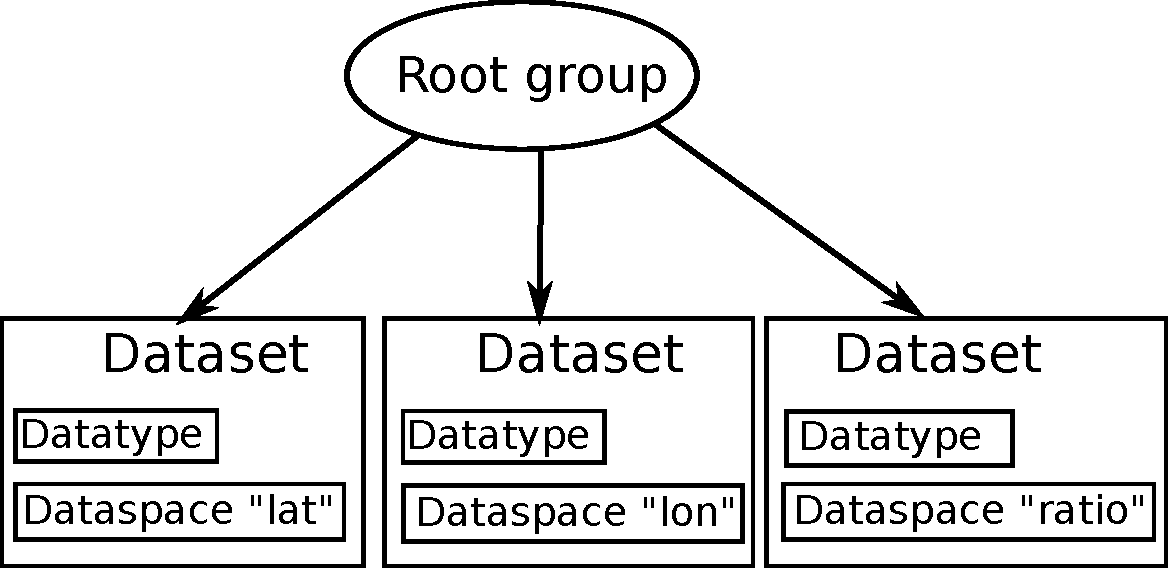
\includegraphics[width=\linewidth]{hdf5.pdf}
    \caption{HDF5 data hierarchy for a simple file in Pangolin, storing the two
      coordinates of the cell center and the tracer ratio. Each data is stored
      in a container (\textit{dataset}), which has data as an 1D array
      (\textit{dataspace}) and  the type of the array (\textit{datatype}), here
      64-bits floats (\textit{H5T\_IEEE\_F64LE}).}
\label{fig:hdf5}
  \end{minipage}  
  \hfill
  \begin{minipage}{0.45\linewidth}
    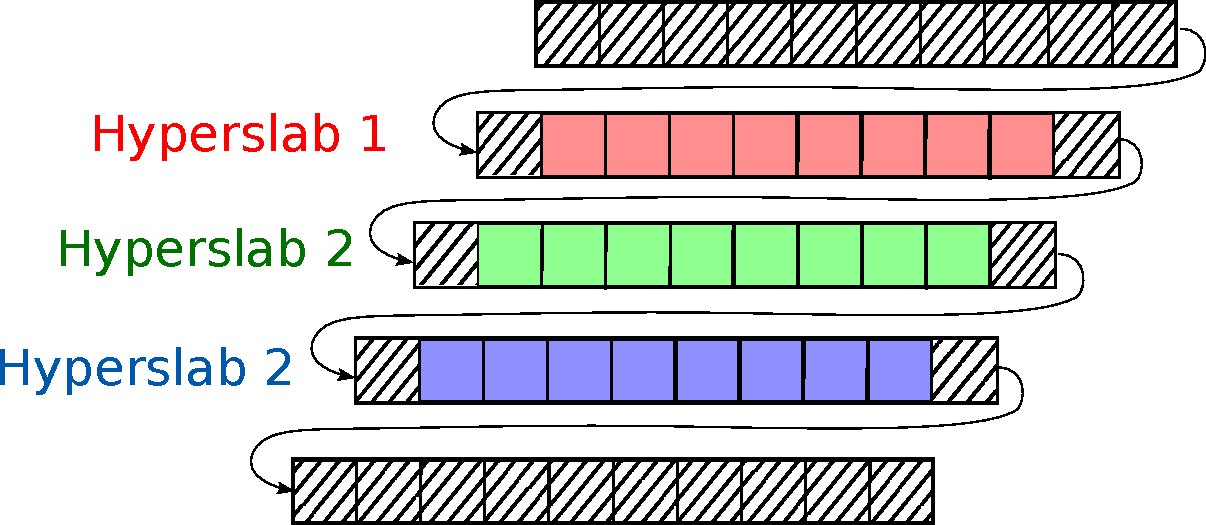
\includegraphics[width=\linewidth]{hdf5_slabs.pdf}
    \caption{Constructing the interior (\textit{i.e}, all non-ghost-cells) of subdomains as
    an union of hyperslabs.  Each hyperslab is defined here by an offset and a
  number of blocks. Ghost cells are shown as hatched.}
\label{fig:hdf5_slabs}
  \end{minipage}  
\end{figure}

\section{Performances}
\label{sec:performances}
\subsection{Configuration}
We now examine the parallel scalability of Pangolin for 2D advection. We focus
on a strong-scaling test, where the total number of cells in the model is
constant, while the number of subdomains increases. The speedup is a common metric
to measure scalability for $n$ cores. Here we take 3 cores as a reference and
define the strong speedup as:
\begin{equation}
  S(n) = \frac{T(3)}{T(n)},
\label{eq:speedup}
\end{equation}
where $T(n)$ is the parallel elapsed time for $n$ cores. In an ideal situation,
$T(n)$ is reduced proportionally to the number of cores so that $S(n) = n/3$. In
practice, we expect communication volume to increase such as the speedup departs
from the ideal situation.

Here, only the elapsed time for advection is measured, \textit{i.e}, the time
spent in Algorithms~\ref{algo:zonal} and~\ref{algo:merid}. As a reference, a
flowchart representing a full run of Pangolin is shown in the Appendix
(Fig.~\ref{fig:pango_run}). Measurements were done on ``Neptune'', the Bull
cluster of the CERFACS\@. Its technical specifications are given on
Fig.~\ref{fig:bull_processor} and~\ref{fig:bull_nodes}. Pangolin was compiled
with the Intel compiler and run using Intel MPI\@.
 
\subsection{Results}
\label{subsec:results} 
A first simulation was run up to 126 cores to study the impact of grid
resolution on scalability. We used the Gaussian hills conditions described in
Section~\ref{subsec:test_cases}, where winds are constant, for a simulation of
12 days. Results are shown on Fig.~\ref{fig:speedup_res}. As expected, the
increase in resolution improves the scalability as the computation workload
grows. Furthermore, the speedup only increases at optimal configurations: namely
6, 24, 54 and 96 cores here. As expected, suboptimal cases uses more cores but
the limiting factor is the size of the largest, \textit{i.e}, slowest,
subdomain, which does not change between optimal values fo the number of MPI
processes.  For a second test, we have ensured the speedup does not change when
advecting multiple species (ten in our test). This confirms that communication
costs are only paid once for all tracers and the cost of pure advection is truly
a linear function of the number of tracers. Therefore, we can assume parallel
performances will scale linearly with the number of tracers.

As a third test, the finest resolution from the first test
($0.28{\degre}\times0.188\degre$) was used to examine the performance of 2D
advection up to 294 cores. Results are presented on Fig.~\ref{fig:speedup_chem}.
At the time being, there is no full chemistry in Pangolin so the impact of
chemistry was estimated using the average cost per cell. This cost was found
using the ASIS chemical solver developed by D.~Cariolle (personal communication,
2014). It solves locally a linear system associated with the integration of an
\gls{ODE} required by the chemical interactions between the 90 species. An
implementation was done by P.~Moinat with the GMRES method, an iterative method
to solve linear systems (\cite{Saad1986}). \\
As a first approximation, the cost of chemistry is constant for all cells so the
estimation was found from the average cost multiplied by the number of cells.
The figures only shows optimal situations, \textit{i.e}, when the number of
cores is of the form $6p^2$.  For truly optimal configurations, we should
require that $p$ divides the number of latitudes in hemisphere. However,
relaxing this constraint only unbalances slightly the load across the subdomains
and allows for a larger choice of the number of cores.  The plot is typical of
parallel MPI applications, where the speedup departs from the linear speedup
when the number of cores increases. As the chemistry is local to each cell, it does
not require any communication volume and only benefits the parallelism, which is
indeed confirmed by the plot. For instance, results at 294 cores give a speedup
of around 72\% of the theoretical speedup for the advection only and rises to
80\% of the theoretical speedup with both advection the estimated chemistry. 

\begin{figure}
  \subbottom[Impact of grid resolution (up to 126 cores).]{%
    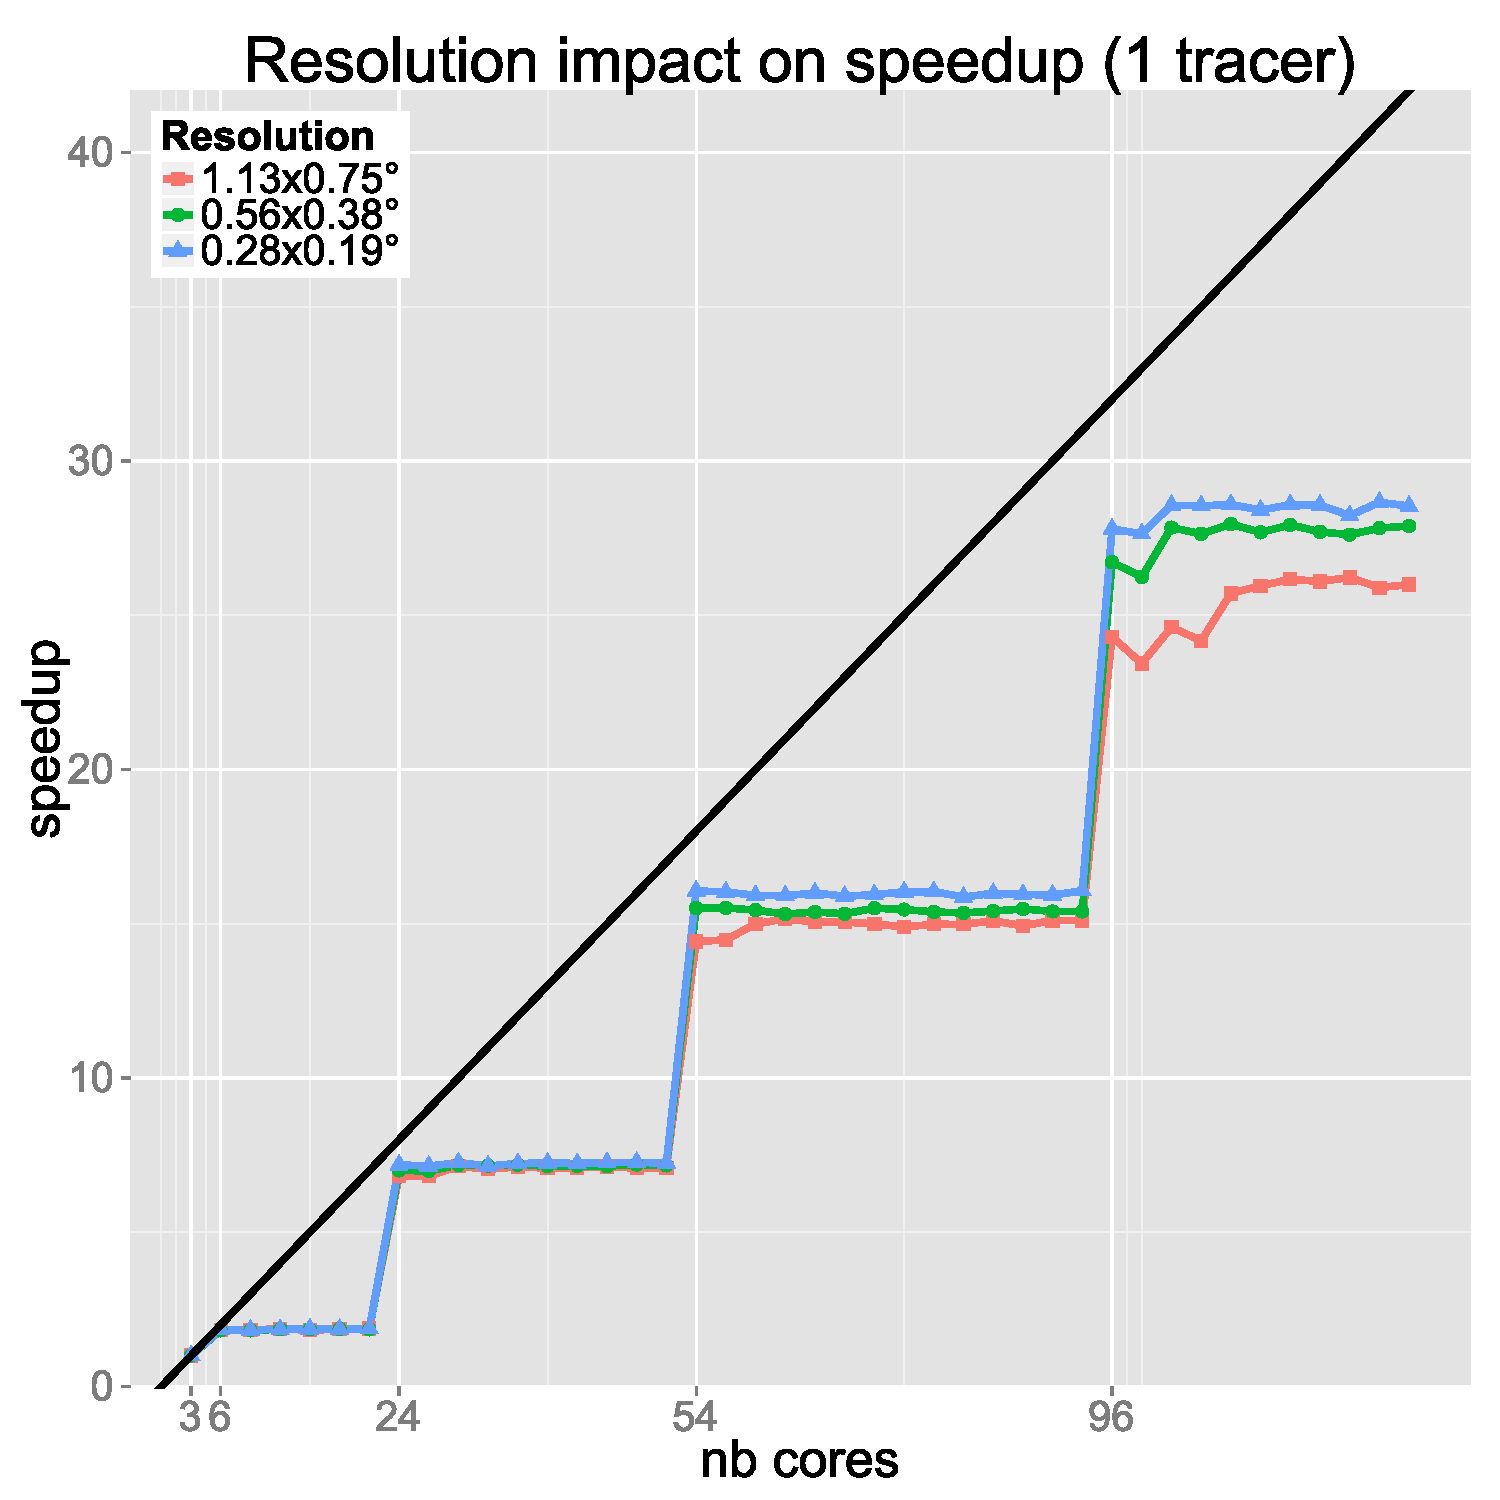
\includegraphics[width=0.49\linewidth]{speedup_resolution.pdf}
\label{fig:speedup_res}}
  \hfill
   \subbottom[Advection performances and an estimation of the
    chemistry impact on scalability.]{%
    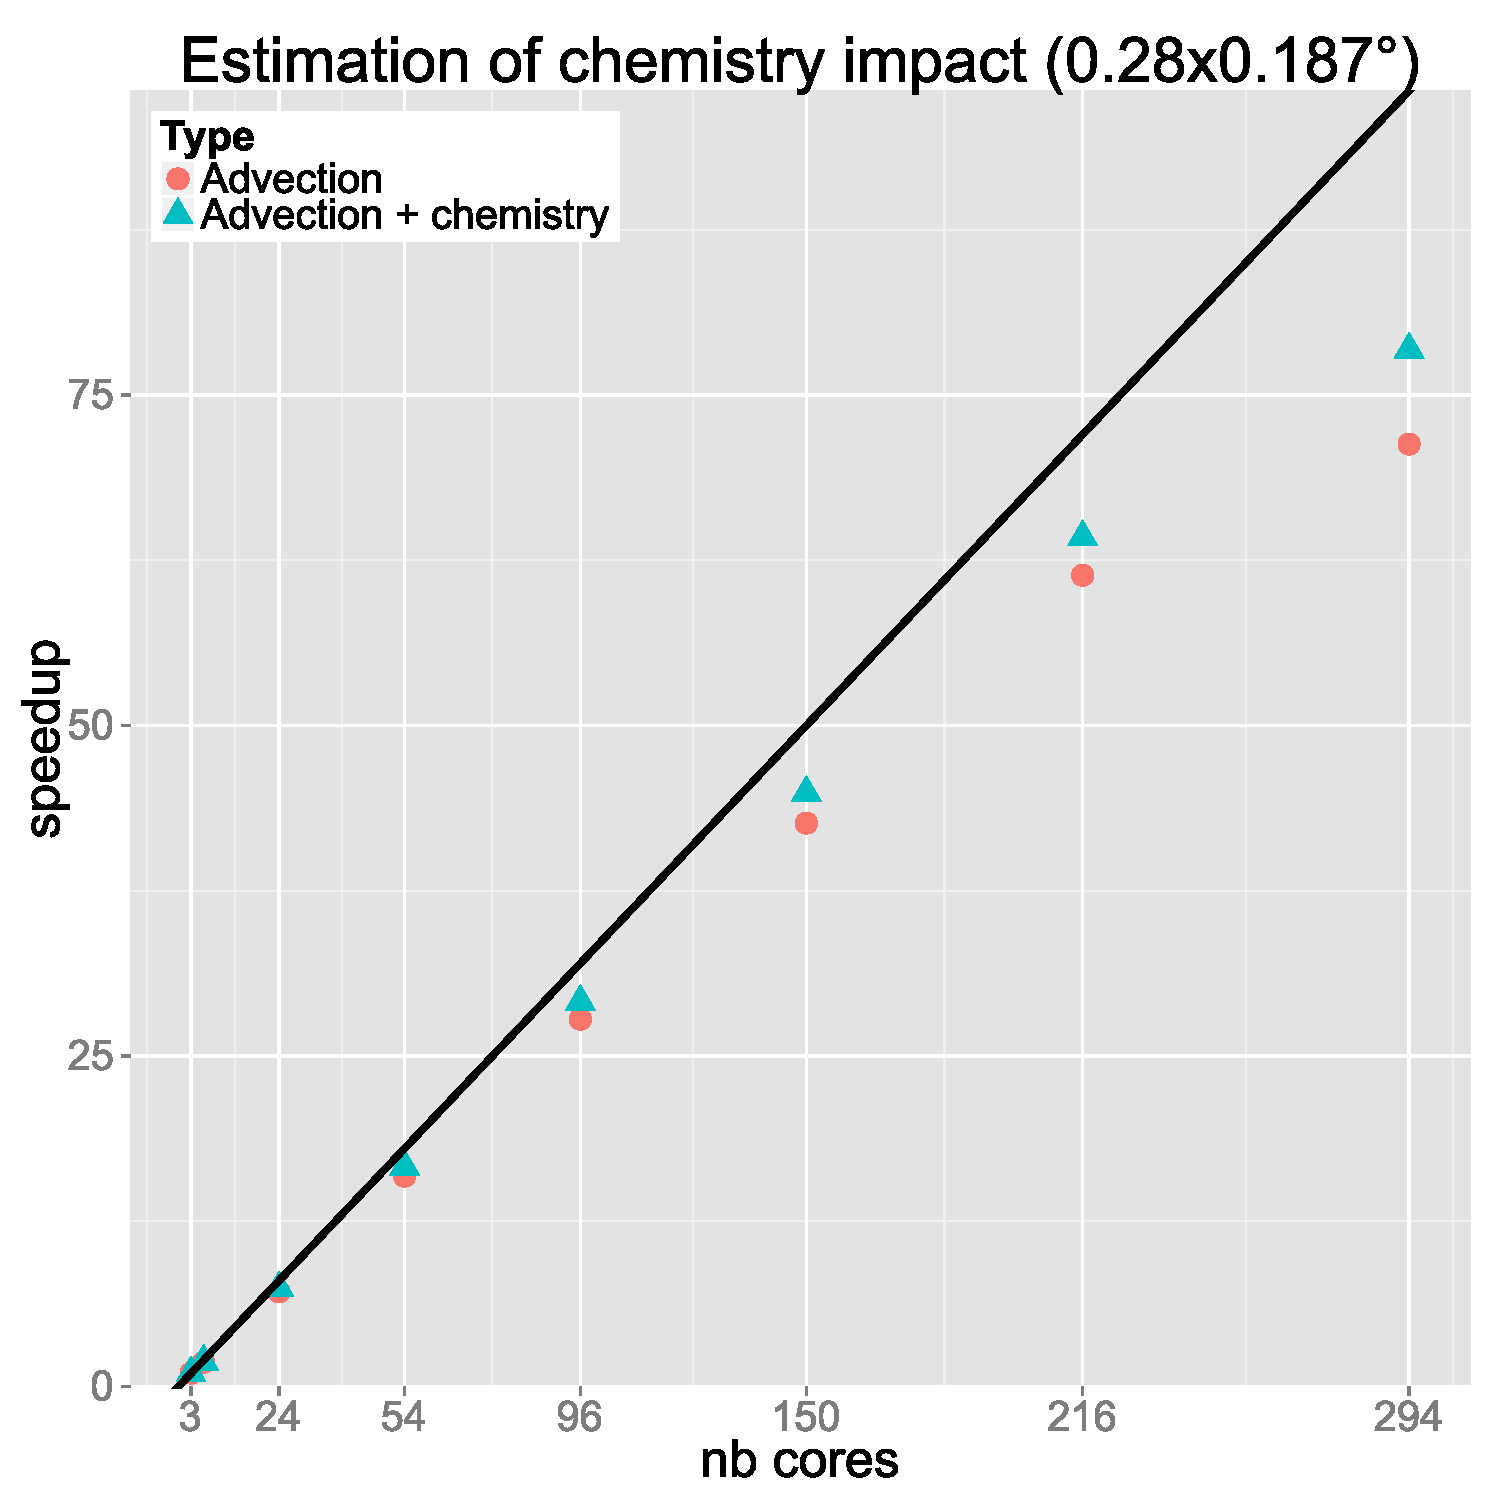
\includegraphics[width=0.49\linewidth]{speedup_chem.pdf}
\label{fig:speedup_chem}}
  \caption{%
    Performance of 2D parallel advection using the speedup defined in
    Eq.~\eqref{eq:speedup}. Resolutions used are:
    $1.125{\degre}\times0.75\degre$, $0.56{\degre}\times0.376\degre$,
    $0.28{\degre}\times0.188\degre$. Both figures use non-divergent winds from
    Section~\ref{sec2:tests} over a~full period with a~CFL of 0.96.
  }
\end{figure}

This leads us to examine the maximal number of cores that can be used for a
given resolution. For that, we chose a rather coarse resolution
($2.25\times1.14\degre$) and increased the number of coarse until the speedup
became too low. This time, we used the Airain supercomputer instead of the
CERFACS cluster (see Table~\ref{tab:cluster_airain} for its main technical features).
Results are shown on Fig.~\ref{fig:efficiency}, which shows \textit{efficiency}
instead of speedup. Efficiency is simply defined as an adimensioned speedup, so
in our case:
\begin{equation}
  E(n) =\frac{T(3)}{nT(n)}
\end{equation}
As such, the closest $E(n)$ is to $1$, the better parallel performances are.  To
understand the results, the x-axis on Fig.~\ref{fig:efficiency} shows the number
of interior cells for meridional fluxes over the total number of interior cells.
For more details, Fig.~\ref{fig:domains_limit} gives the ratio of ghost cells
over interior cells. For advection only, we can
consider efficiency is too low below $0.5$, \textit{i.e}, for 150 cores.
This corresponds to subdomains of $8\times8$ cells, where roughly
$44\%$ of the cells are ghost cells. Such subdomains are obviously too small
for practical purposes and only represent a waste of the memory of the node.
This shows the performances of the parallel advection, which only `breaks' down
for such small subdomains. On top of that, we estimate the chemistry will more
than double this maximal number of cores, as for 294 cores, the total efficiency
is estimated at $0.75$.

\begin{table}[t]
\caption{Configuration of the Bull cluster Airain}
\centering
\begin{tabular}{l}
\toprule
-- 549 nodes Bullx B510\\
-- 9504 cores Intel SandyBridge\\
-- each node has 16 cores at 2.7Ghz and 4GB shared by the core\\
\bottomrule
\end{tabular}
\label{tab:cluster_airain}
\end{table}

\begin{figure}
  \subbottom[Efficiency for advection and with an estimation of the cost of
    chemistry.]{%
    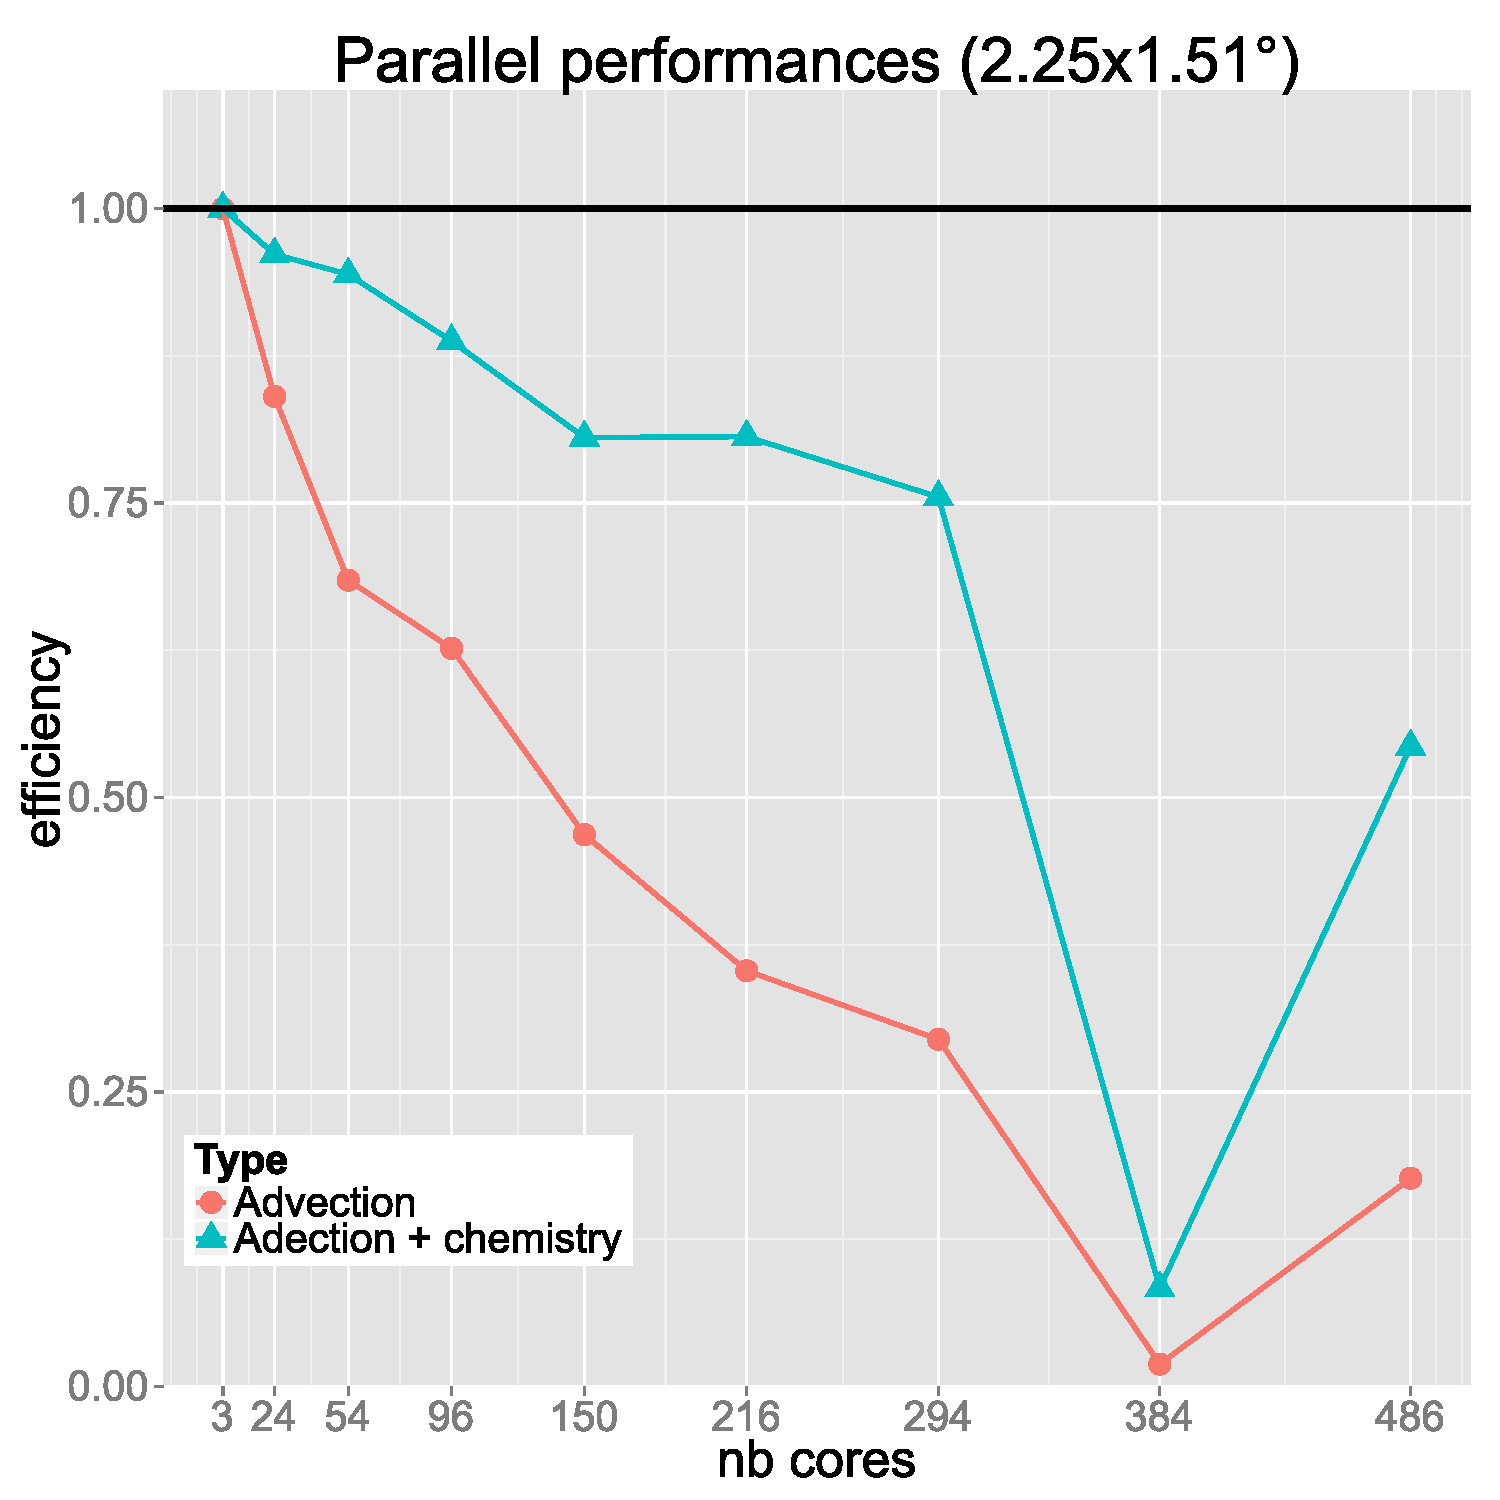
\includegraphics[width=0.48\linewidth]{efficiency_limit.pdf}
\label{fig:efficiency}}
  \hfill
   \subbottom[Proportion of ghost and interior cells for a subdomain and for
     meridional fluxes. The number of cores is not linear.]{%
    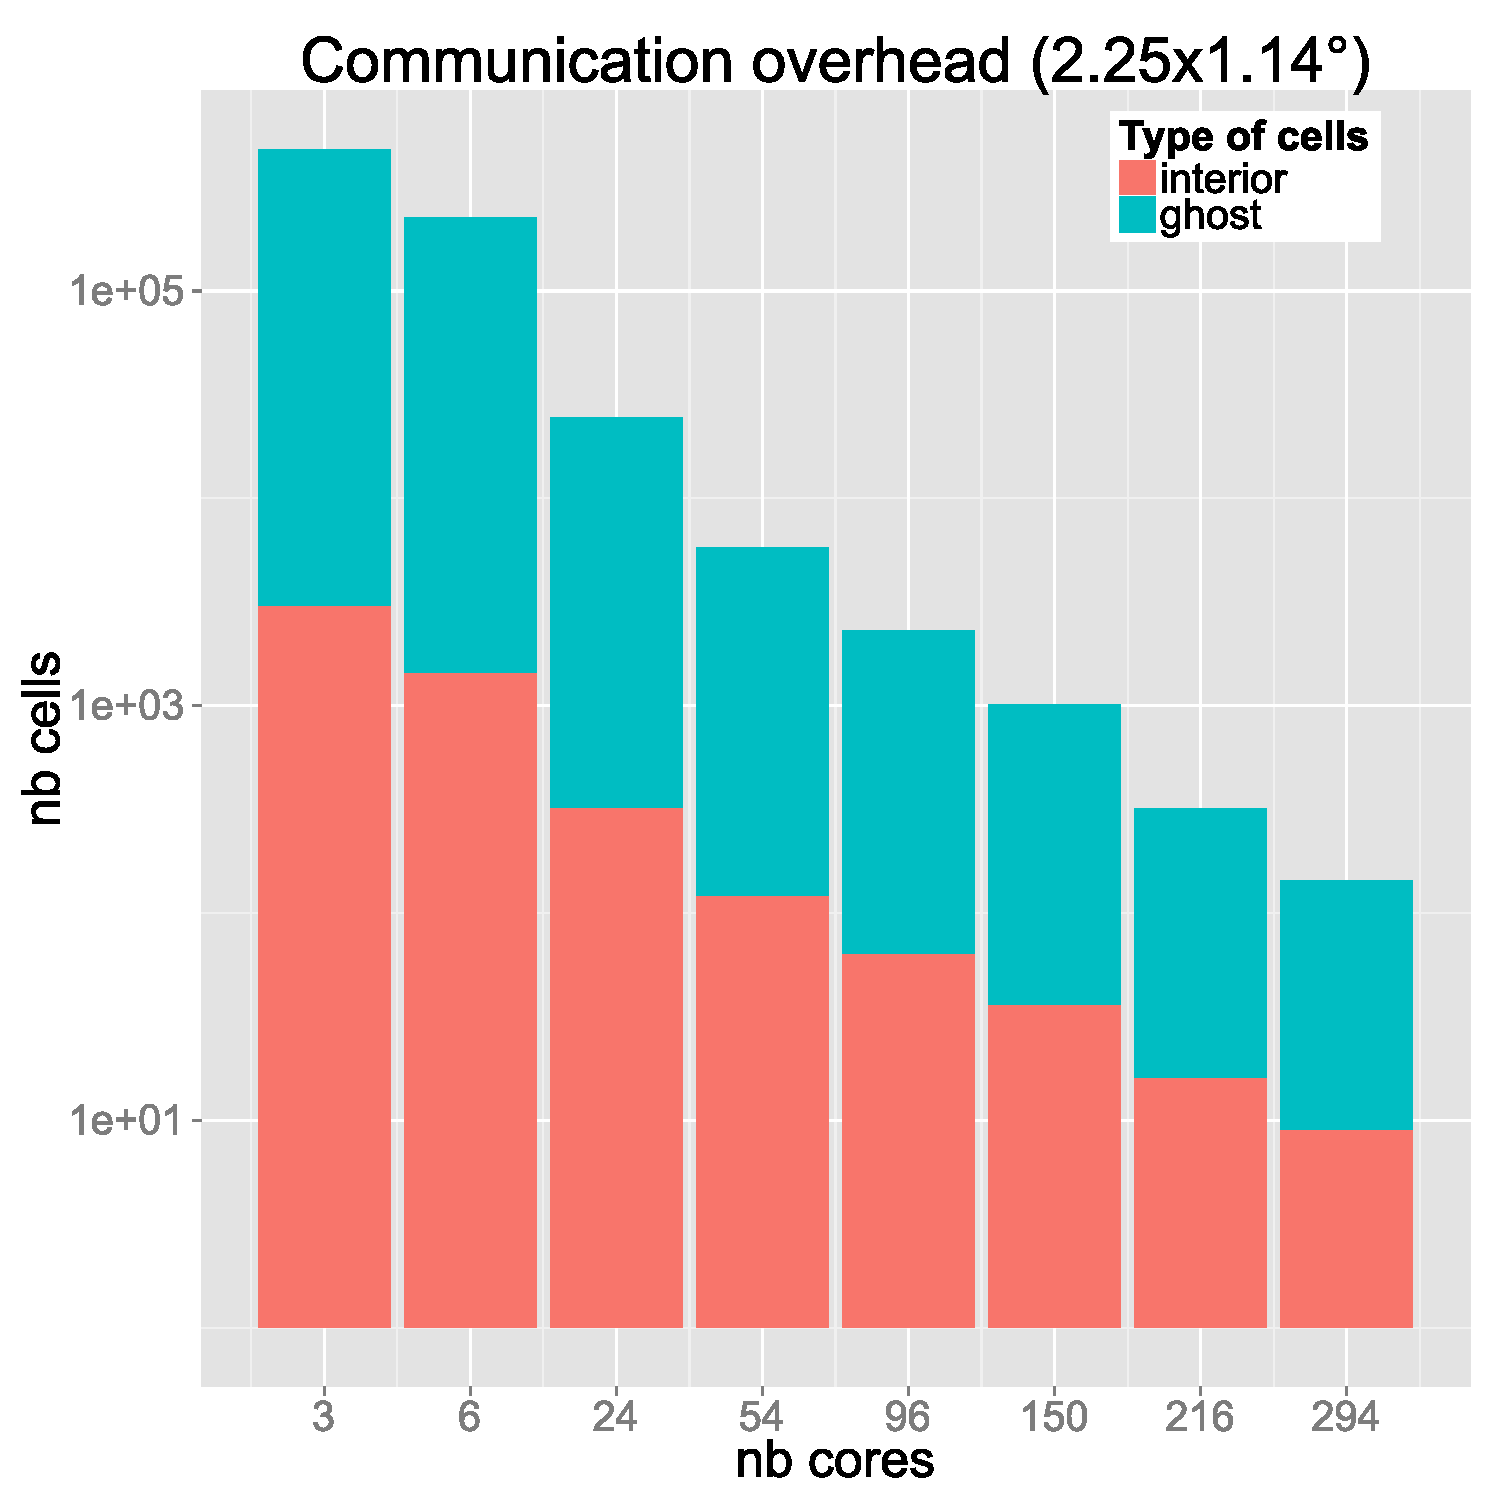
\includegraphics[width=0.48\linewidth]{domains_limit.pdf}
\label{fig:domains_limit}}
  \caption{%
    Impact of communication overhead on parallel performance (2D advection)
    using the Airain supercomputer. The simulation was run with a coarse
    resolution ($2.25\times1.14\degre$) until the performances broke
    down. Only perfect cases for our partitioning were considered.}
\end{figure}

\section{Future work}
\label{sec:future_work}
This chapter only dealt with 2D advection, on which our parallelizaton strategy is
based on.  In the next chapter, a linear scheme for ozone is presented, to test
Pangolin in a ``real-life'' scenario. However, chemical schemes are more complex
in practice and require to solve stiff linear systems. As such, the chemistry
step is much more expensive than pure 2D advection. From a parallelism point of
view, we expect the increase in the computational load to improve speedup. On
the negative side, we expect load balance to be disturbed by heterogeneous
chemistry, surface emissions, as well as convection, vertical diffusion and the
day/night interface.  Extension to the 3D case for advection should also be
beneficial for parallel performances. The idea is to use the 2D domain
decomposition and extend it vertically so a subdomain is a set a vertical
columns. It is not uncommon to have around 60 vertical levels so the
computational workload for advection should be multiplied by 60. 

Here we presented a static load-balancing strategy based on a domain
decomposition strategy. To mitigate the future load unbalancing, a dynamic
strategy can be a solution. A first approach would be to use a hybrid programming
paradigm with MPI and OpenMP, where a varying number of threads would be added
on top of the MPI processes to manage the load unbalance. Another solution would
be to split each subdomain into several subdomains and to assign a thread to it.
However, this would require a domain decomposition strategy, as complex as the
one developed for MPI\@. A third possibility is to exploit suboptimal
configurations in the number of cores. As parallel performance is similar to the
closest lower optimal case, the number of cores for advection could be decreased
and the now idle cores could be stealing work from these
`master' processes.
